This section is devoted to a specific description of every kind of requirement the system has to deal with in order to achieve all the functionalities described.


\section{ External Interface Requirement}
\label{sec:external_interface_requirements}%


\subsection{User interfaces}
\label{subsec:User_interfaces}%


The S\&C's user interface will be a website, developed in order to be used by all the possible users (Universities, Students and Companies).
The following images provide a high-level overview of the interfaces, offering a glimpse into their structure and functionality. A detailed analysis of these interfaces will be presented in the Design Document.

\newpage

\paragraph{Access Page:} When a user navigates to the website for the first time, the access page serves as the initial interface. Here, users are prompted to log in using their credentials. If the user does not already have an account, they are provided with an option to register and create a new one. Additionally, universities can also access this page to proceed with their specific login or registration process, ensuring seamless on-boarding for both individual users and institutional entities.

\begin{figure}[H]
    \begin{center}
        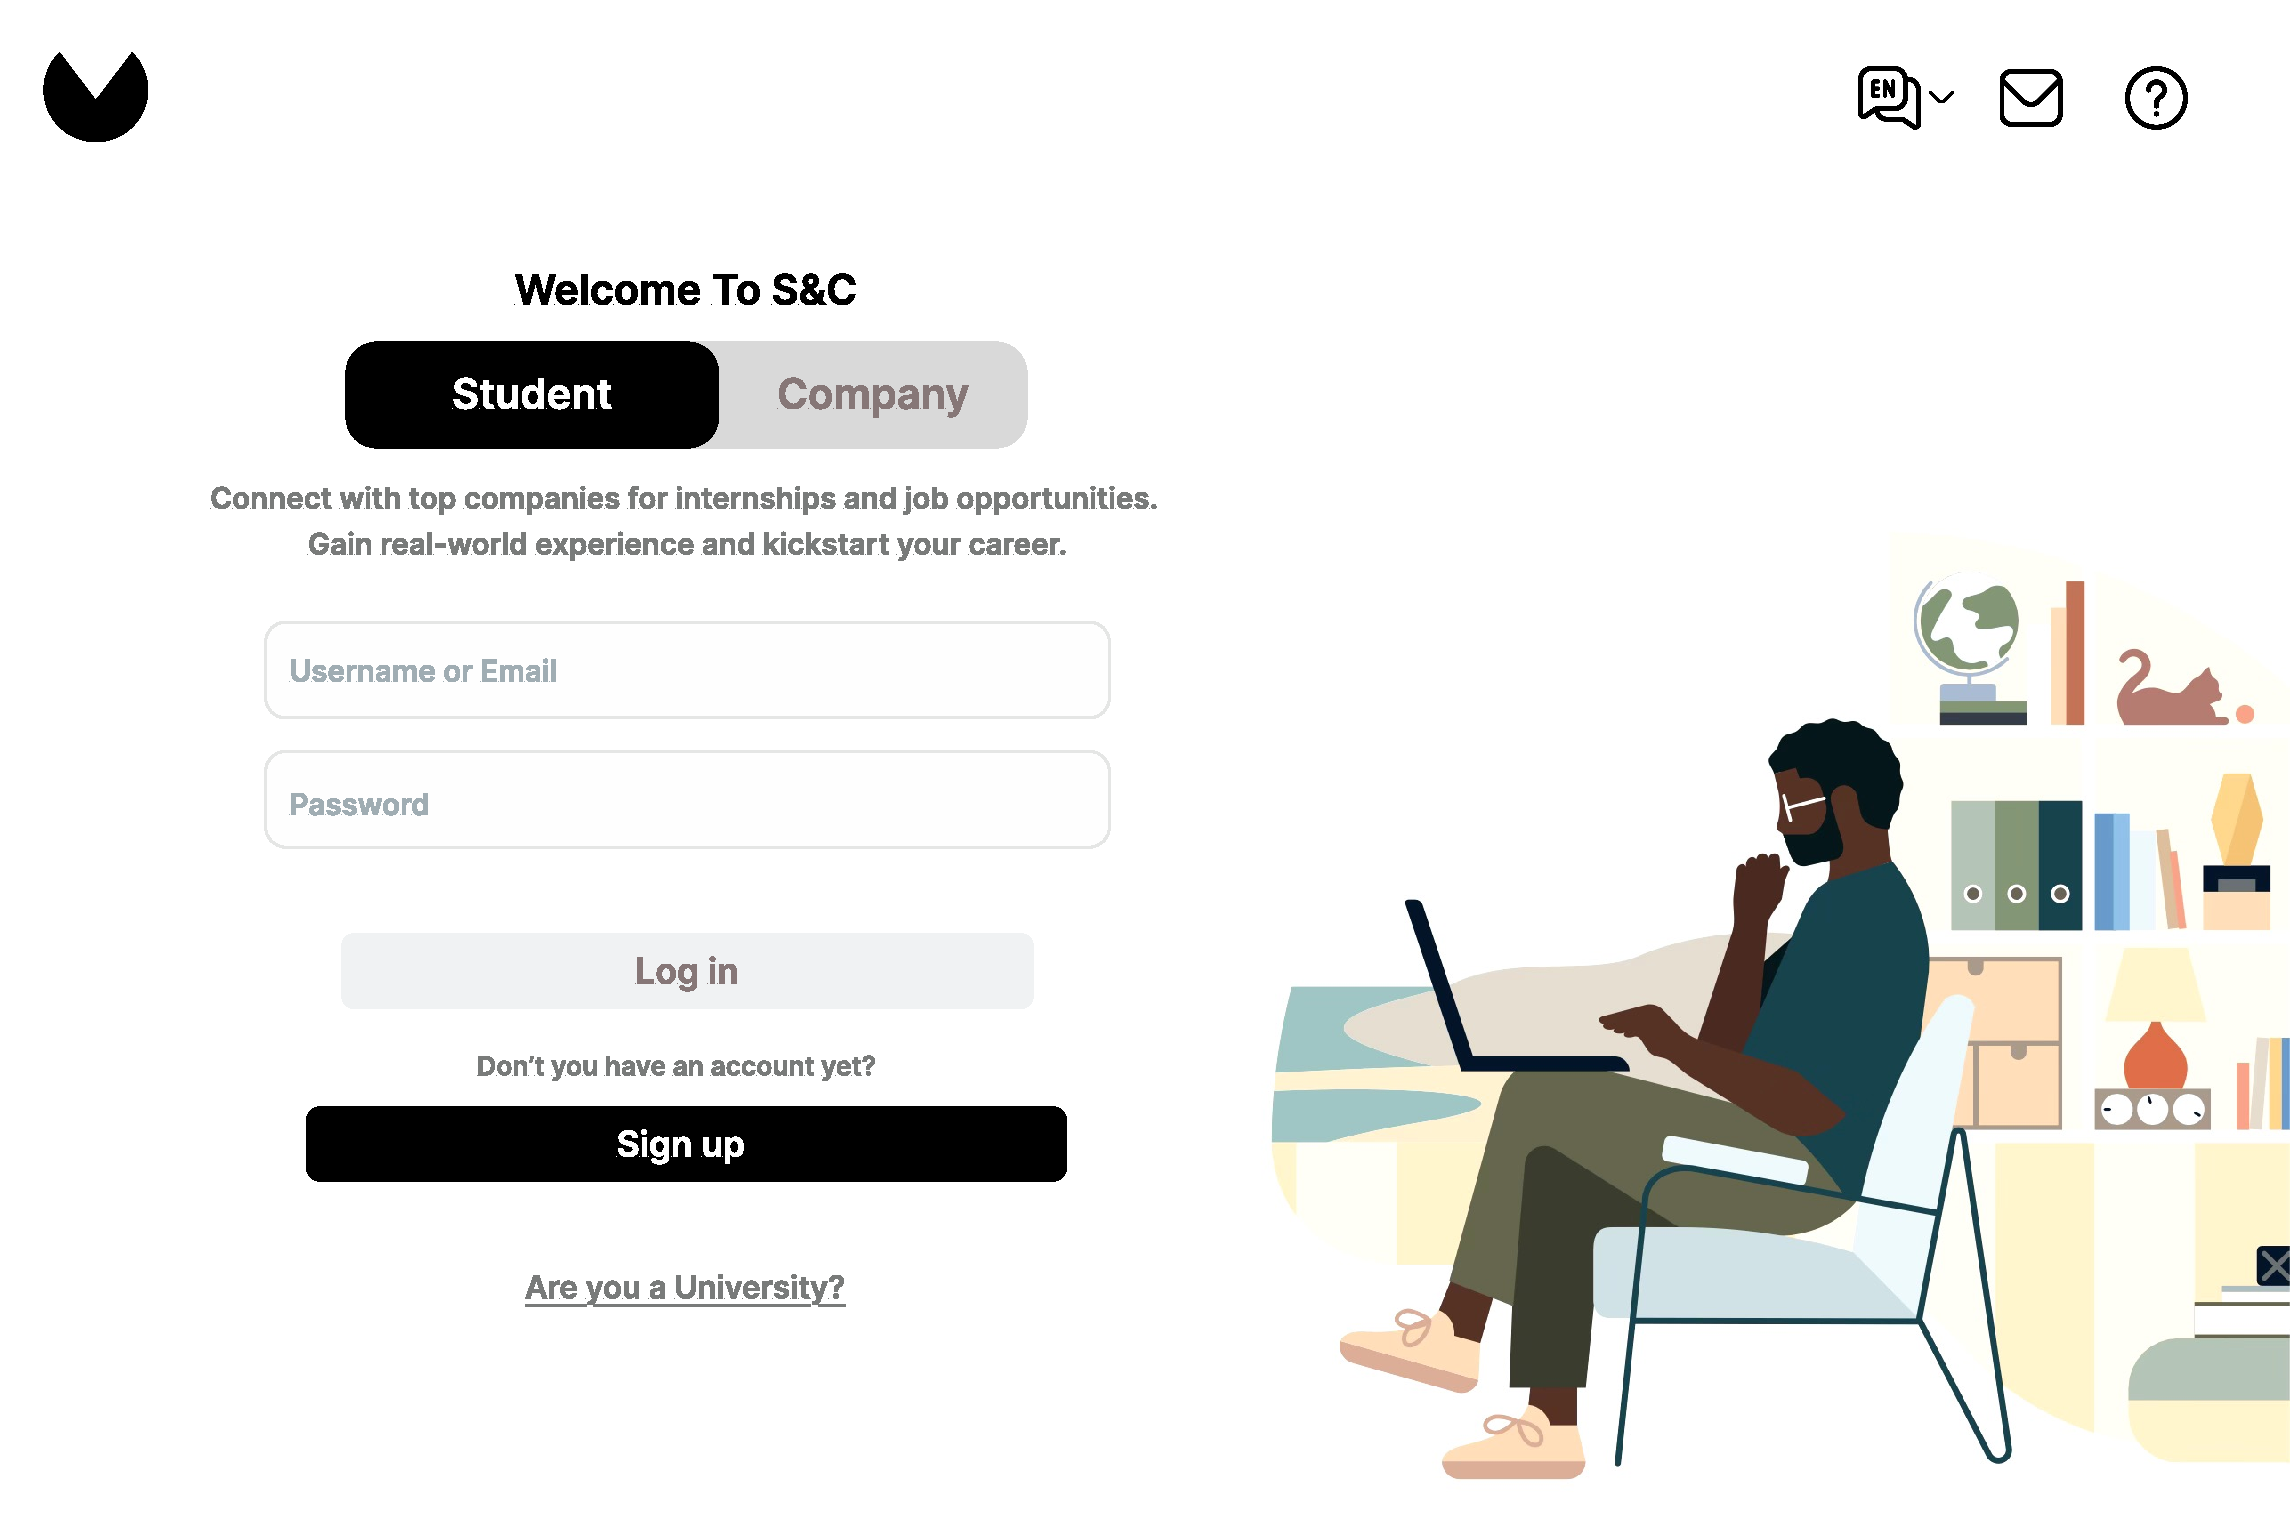
\includegraphics[width=\linewidth]{Images/UserInterfaces/AccessPage.pdf}
        \caption{Access Page UI.}
        \label{fig:access_page_UI}%
    \end{center}
\end{figure}

\newpage

\paragraph{Student Homepage:} When a student enters the homepage, they are greeted with an organized layout. On the left side, an overview of their profile is displayed, along with a section highlighting past and upcoming events. On the right side, a toolbar is provided for searching companies, complemented by an overview of recommended companies. At the top of the page, a small toolbar houses icons for easy access to the homepage, chat, notifications, help, settings, and the student’s personal profile.

\begin{figure}[H]
    \begin{center}
        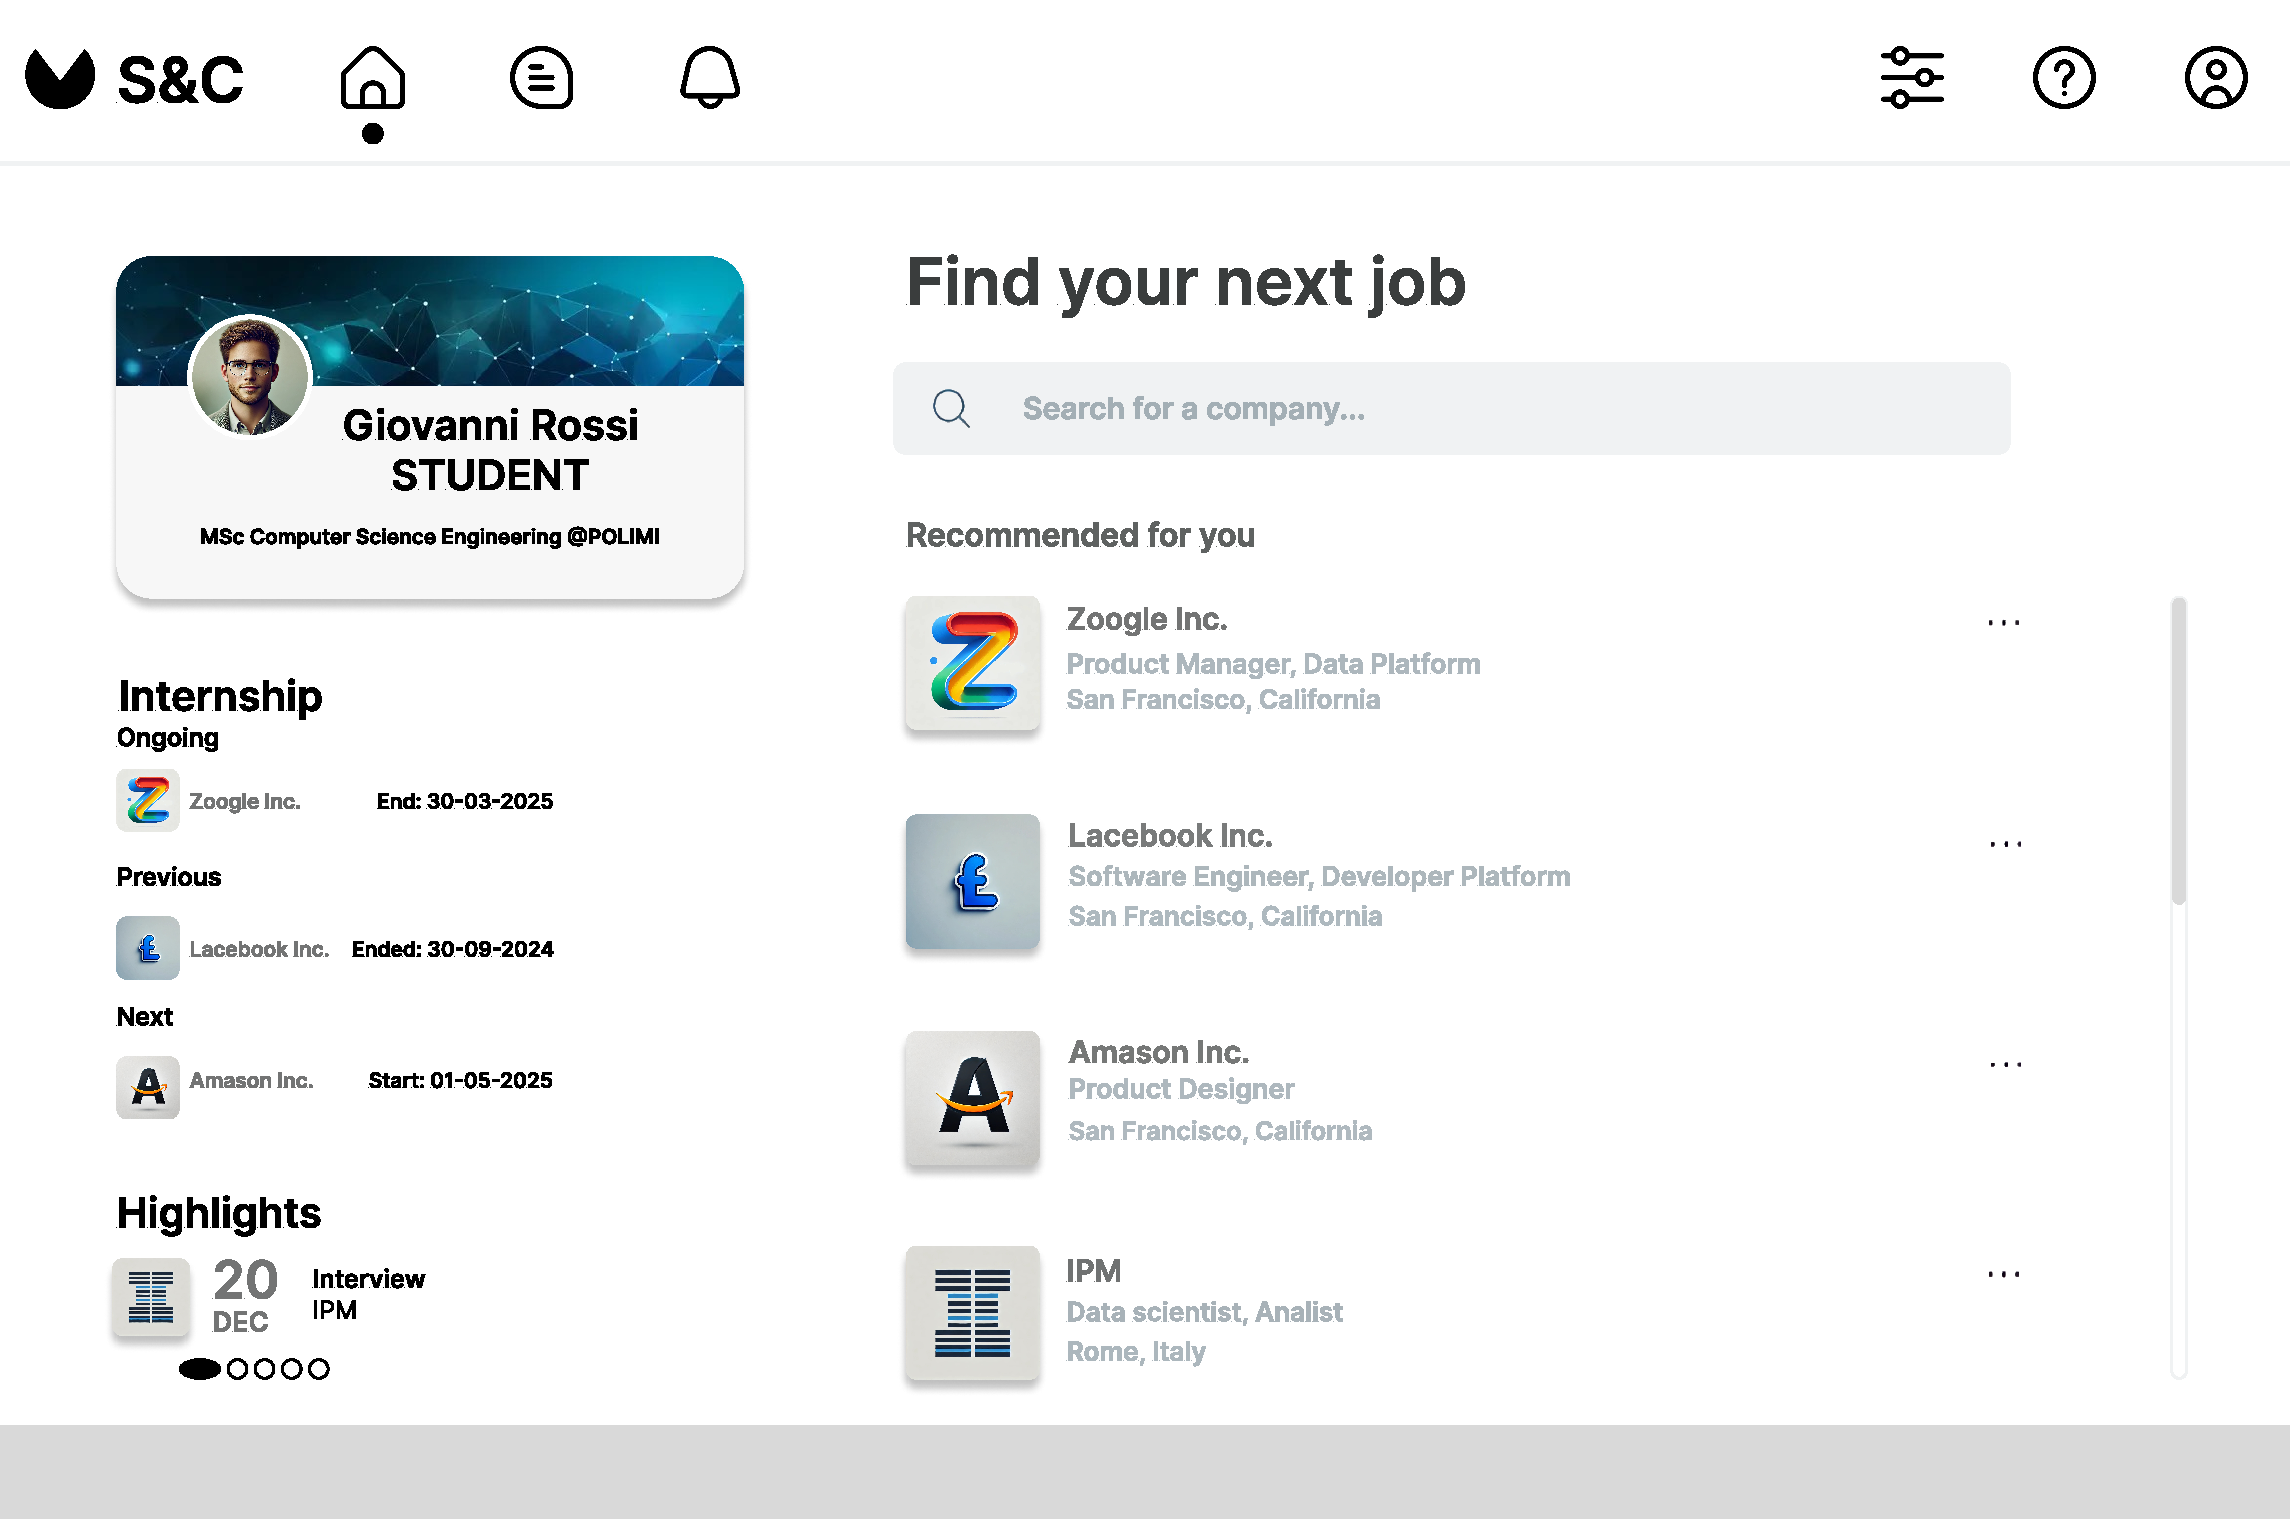
\includegraphics[width=\linewidth]{Images/UserInterfaces/SHomepage.pdf}
        \caption{Student Homepage UI.}        
        \label{fig:student_homepage_UI}%
    \end{center}
\end{figure}

\newpage

\paragraph{Chat page:} When a user navigates to the chat page, they are presented with a clear layout. On the left side, a list of open chats is displayed, allowing quick access to previous conversations. On the center-right side, the selected chat appears, featuring a text input bar, a send button, and a "+" button for additional operations, such as adding information, submitting a complaint, and other actions only for companies.

\begin{figure}[H]
    \begin{center}
        \includegraphics[width=\linewidth]{Images/UserInterfaces/SChatpage.pdf}
        \caption{Chat Page UI.}
        \label{fig:chat_page_UI}%
    \end{center}
\end{figure}

\newpage

\paragraph{Notifications page:} When the user accesses the notifications page, they are presented with a list of notifications they have received, ordered from the most recent to the least. This provides an easy way to stay up-to-date with important alerts and messages.

\begin{figure}[H]
    \begin{center}
        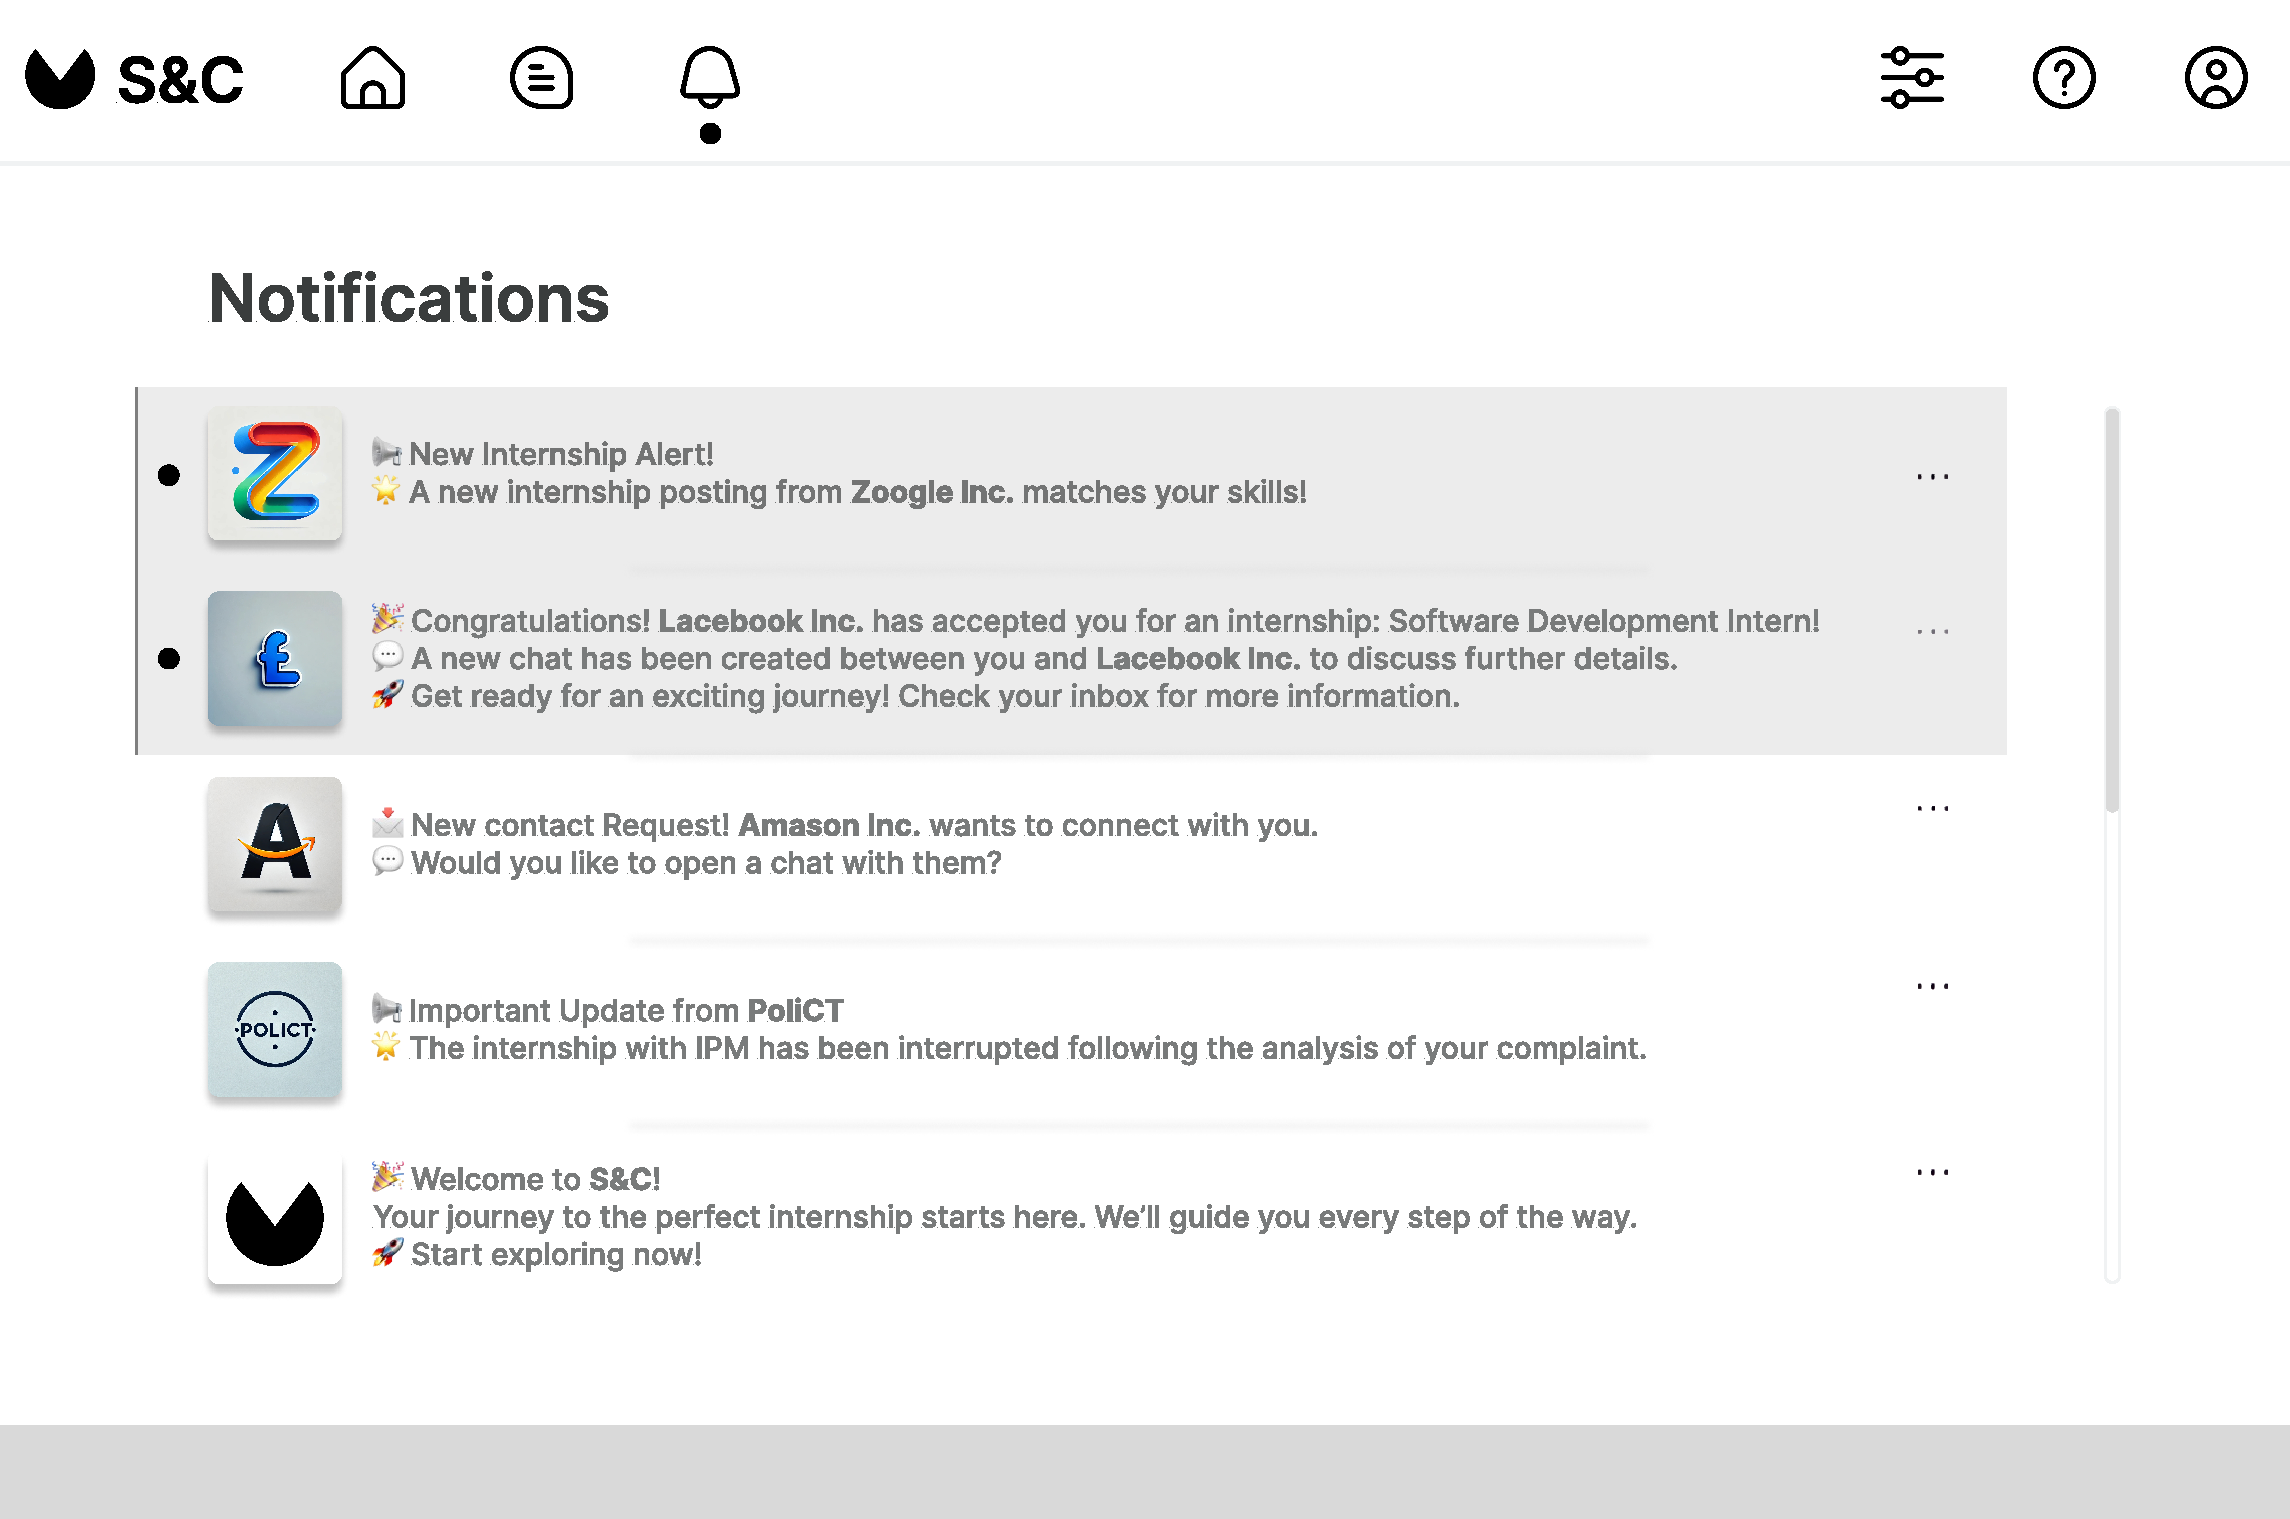
\includegraphics[width=\linewidth]{Images/UserInterfaces/NotificationPage.pdf}
        \caption{Notifications Page UI.}
        \label{fig:notifications_page_UI}%
    \end{center}
\end{figure}


\subsection{Hardware interfaces}
\label{subsec:hardware_interfaces}%


The system will be accessible from any device equipped with an internet
browser and a stable internet connection. Users can choose their
preferred device, such as a computer, tablet, or smartphone. However, it
is recommended to use a computer for a more seamless experience when
navigating through the internship postings.


\subsection{Software interfaces}
\label{subsec:software_interfaces}%


The S\&C platform requires integration with the following software
interfaces to function effectively:

\begin{enumerate}
\def\labelenumi{\arabic{enumi}.}
\item
  \textbf{Email Provider}:\\
  The platform will utilize an eMail provider (e.g., SMTP) to send
  confirmation eMails during user registration, as well as notifications
  for internship matches, updates, and reminders.
\item
  \textbf{Notification System}:\\
  A built-in notification mechanism will deliver real-time updates to
  users within the platform (e.g., dashboard notifications for new
  applications or interview schedules).
\item
  \textbf{Data Analytics Services}:\\
  To enhance recommendations and feedback analysis, the platform may
  connect with analytics APIs or modules for data-driven insights.
\end{enumerate}

These software interfaces ensure seamless communication, efficient
notifications, and smooth external tool integration for a better user
experience.


\subsection{Communication interfaces}
\label{subsec:communication_interfaces}%


The communication interfaces required by the S\&C platform are as
follows:

\begin{enumerate}
\def\labelenumi{\arabic{enumi}.}
\item
  \textbf{HTTPS Protocol}:\\
  The platform will use HTTPS to ensure secure communication between
  users and the system, encrypting all data exchanged to protect user
  privacy and information.
\item
  \textbf{SMTP (Simple Mail Transfer Protocol)}:\\
  The platform will utilize SMTP for sending emails, including
  confirmation emails during registration, notifications about
  internship opportunities, application statuses, interview schedules,
  and other important updates to users.
\end{enumerate}

These communication interfaces are essential to ensure secure data
transmission and reliable email functionality within the system.


\section{Functional requirements}
\label{sec:functional_requirements}%


\subsection{Requirements}
\label{subsec:requirements}%


Here is the list of functional requirements organized by user classes:


\textbf{Guest}

{[}R1{]}: The system should allow an unregistered guest to sign up.

\textbf{Student}

{[}R2{]}: The system should allow registered students to log in.

{[}R3{]}: The system should allow students to insert their CVs and
manage their profile information (e.g. personal data, skills and profile
photo).

{[}R4{]}: The system should provide personalized suggestions to students
for enhancing their CVs to improve their chances of being selected.

{[}R5{]}: The system should notify students when internships matching
their skills, experiences, and interests become available.

{[}R6{]}: The system should allow students to browse available
internship postings.

{[}R7{]}: The system allows S to visualize the profile of other C.

{[}R8{]}: The system should allow S to submit applications for specific
internship postings.

{[}R9{]}: The system should allow S to provide feedback, suggestions and
rating to improve the recommendation process.

{[}R10{]}: The system allows S to establish a contact with C when mutual
interest is identified.

{[}R11{]}: The system should assist S in scheduling interviews.

{[}R12{]}: The system should allow S to track the status of their
applications and final selections.

{[}R13{]}: The system should provide S with a mechanism to report issues
or complaints related to ongoing internships.

{[}R14{]}: The system should allow S to review the S\&C Calendar.

{[}R15{]}: The system should insert the S's events on the S\&C Calendar.

\textbf{Company}

{[}R16{]}: The system should allow registered companies to log in.

{[}R17{]}: The system should allow C to manage their organization
profile.

{[}R18{]}: The system should allow C to post new internship
opportunities, specifying details such as required skills, tasks, and
benefits.

{[}R19{]}: The system should provide suggestions to C to improve their
internship postings, making them more appealing to S.

{[}R20{]}: The system allows C to visualize the profile of other Users.

{[}R21{]}: The system should inform C about the availability of S CVs
corresponding to their needs.

{[}R22{]}: The system should allow C to provide feedback and suggestions
to improve the recommendation process.

{[}R23{]}: The system allows C to establish a contact with S when mutual
interest is identified.

{[}R24{]}: The system should enable C to track the progress of their
internship selection processes, including applications and decisions.

{[}R25{]}: The system should allow C to submit complaints or information
related to internships.

{[}R26{]}: The system should allow C to review the S\&C Calendar.

{[}R27{]}: The system should insert the C's events on the S\&C Calendar.

\textbf{University}

{[}R28{]}: The system should allow U to log in.

{[}R29{]}: The system should allow U to monitor internships of their
students.

{[}R30{]}: The system should allow U to interrupt ongoing internships.


\subsection{Use case diagrams}
\label{subsec:use_case_diagrams}%


\begin{figure}[H]
    \begin{center}
        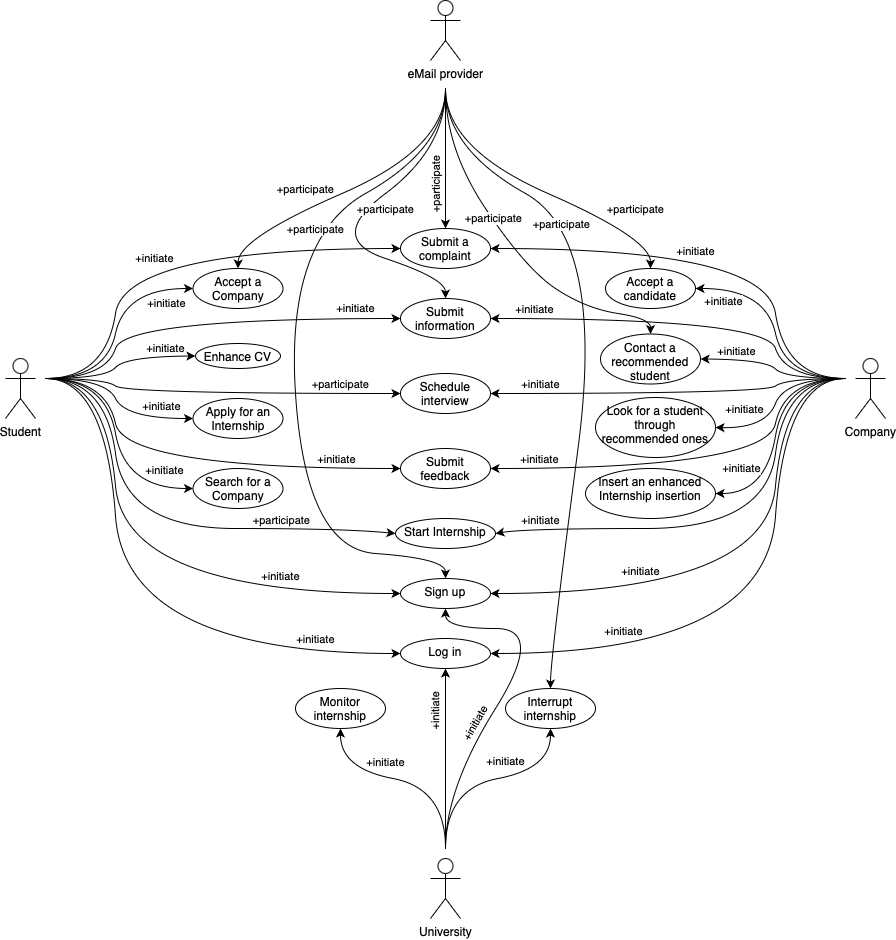
\includegraphics[width=\linewidth]{Images/UCDiagram.png}
        \caption{Use Cases Diagram for all the Users.} 
        \label{fig:UnregisteredUC}%
        \end{center}
\end{figure}


\subsection{Use cases}
\label{subsec: use_cases}%
\newcounter{uc}
\setcounter{uc}{1}
\newcommand{\cuc}{\theuc\stepcounter{uc}}

This chapter presents core use cases, showcasing the application's real-world impact and versatility.

\subsubsection*{UC\cuc . Sign Up}
\begin{center}
    \begin{longtable}{|l|p{0.75\linewidth}|}
        \hline
        \textbf{Name}               & Sign Up\\
        \hline
        \textbf{Actor}              & Guest, eMail provider\\
        \hline
        \textbf{Entry conditions}   & The Guest wants to create an account and knows the S\&C URL\\
        \hline
        \textbf{Event Flow}         & 1 - The Guest enters the URL of S\&C on the search bar of his browser.    \\
        & 2 - The Guest clicks on the “Sign Up” button entering in the registration page.    \\
        & 3 - The Guest selects the correct registration form by selecting the right option between Student, Company or University. \\
        & 4 - The Guest enters his personal information: eMail, password, name and username for the S; eMail, password, name, VAT Name and username for the C; eMail, password, name, PEC, Name and username for the U. \\
        & 5 - The Guest clicks on the “Accept \& Join” button.  \\
        & 6 - The system checks the credentials.    \\
        & 7 - If the check is successful the system sends a confirmation eMail to the User through the eMail provider.  \\
        \hline
        \textbf{Exit condition}   & The system lets the User enter the website. \\       
        \hline
        \textbf{Exceptions}       & \begin{itemize}
            \item The username is already in use, so the system shows an error message and the registration form is shown again.
            \item The eMail is already in use, so the system shows an error message and the registration form is shown again.
            \item The password is not valid: it’s less than 8 characters long and/or it doesn’t contain any uppercase letter and/or it doesn’t contain any lowercase letter and/or it doesn’t contain any number and/or it doesn’t contain any special character (!,\#,\&,\$,?,+,-). The system shows an error message and the registration form is shown again.
        \end{itemize}\\
        \hline
        \caption{Sign Up use case.}
        \label{tab: sign_up_use_case}
    \end{longtable}
\end{center}


\begin{figure}[H]
    \begin{center}
        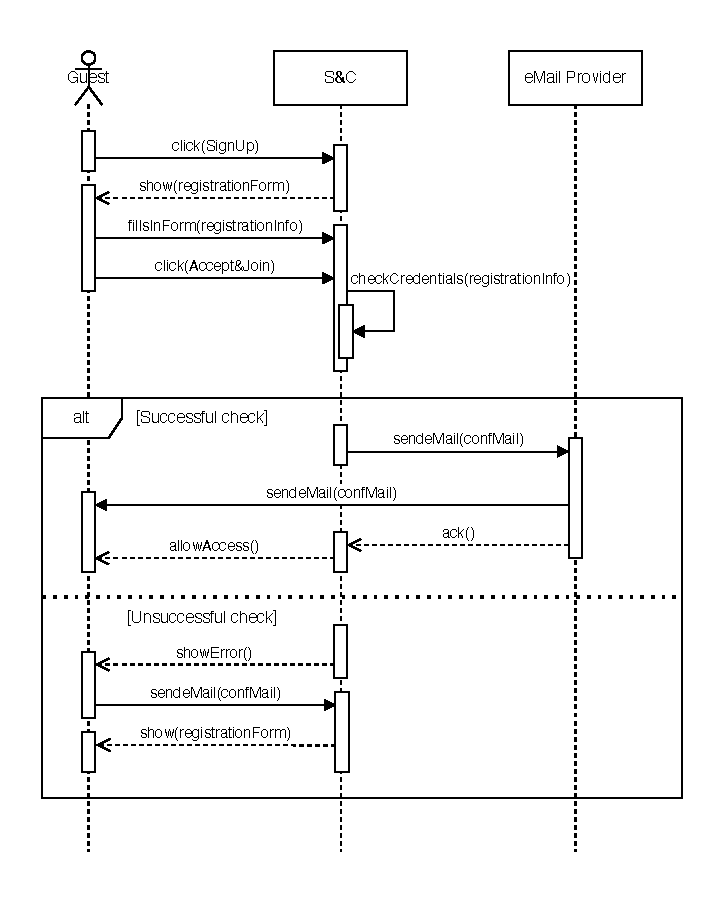
\includegraphics[width=\linewidth]{Images/SequenceDiagram/SignUpSD.pdf}
        \caption{Sign Up sequence diagram.}
        \label{fig:sign_up_seqdiag}%
    \end{center}
\end{figure}


\subsubsection*{UC\cuc . Login}
\begin{center}
    \begin{longtable}{|l|p{0.75\linewidth}|}
        \hline
        \textbf{Name}               & Login\\
        \hline
        \textbf{Actor}              & Users\\
        \hline
        \textbf{Entry conditions}   & The Guest wants to access his account\\
        \hline
        \textbf{Event Flow}         & 1 - The Guest enters the URL of S\&C on the search bar of his browser.    \\
        & 2 - The Guest selects the right option between Student and Company button or in the case of a University clicks on the “Are you a University?” button. \\
        & 3 - The Guest enters the email and password in the correct form. \\
        & 4 - The Guest clicks on the “Login” button. \\
        & 5 - The system checks the credentials. If the check is successful it redirects the user to the right main page, according to his role.  \\
        \hline
        \textbf{Exit condition}   & The User is logged in and can surf into the website. \\       
        \hline
        \textbf{Exceptions}       & \begin{itemize}
            \item Incorrect eMail or password. An error message is shown and the User is redirected back to the Login page.
        \end{itemize}   \\
        \hline
        \caption{Login use case.}
        \label{tab: login_use_case}
    \end{longtable}
\end{center}


\begin{figure}[H]
    \begin{center}
        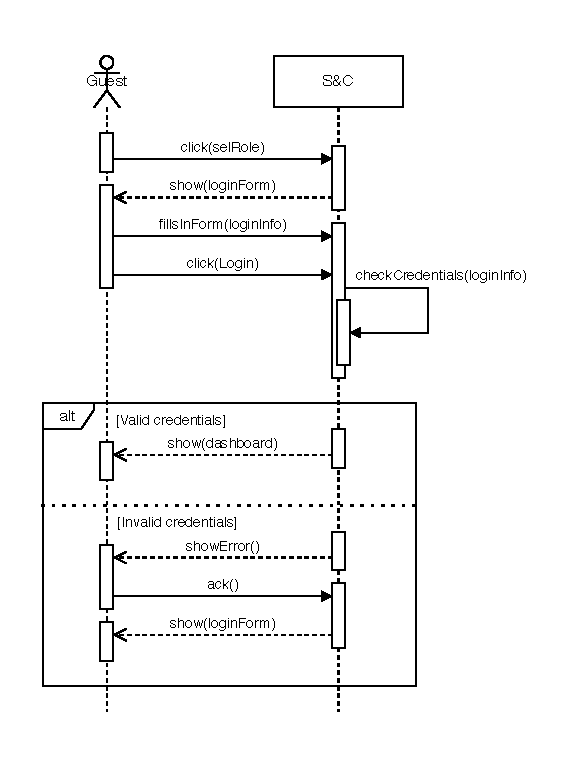
\includegraphics[width=\linewidth]{Images/SequenceDiagram/LoginSD2.pdf}
        \caption{Login sequence diagram.}
        \label{fig:login_seqdiag}%
    \end{center}
\end{figure}


\subsubsection*{UC\cuc . Insert an enhanced Internship Insertion}
\begin{center}
    \begin{longtable}{|l|p{0.75\linewidth}|}
        \hline
        \textbf{Name}               & Insert an enhanced Internship Insertion\\
        \hline
        \textbf{Actor}              & C\\
        \hline
        \textbf{Entry conditions}   & The C is logged in and wants to post a new insertion.\\
        \hline
        \textbf{Event Flow}         & 1 - The C clicks on “Post” at the bottom-right of his homepage. \\i
        & 2 - The C fills in the forms with all the information needed about his position. \\
        & 3 - The C clicks on the “Enhance” button. \\
        & 4 - The system analyzes the insertion and gives suggestions on how to improve project description. \\
        & 5 - The C reviews the suggestions given by the system and modifies the insertion if needed. \\
        & 6 - The C clicks on the “Post” button. \\
        \hline
        \textbf{Exit condition}   & The system publishes the C’s insertion and shows to the C his homepage. \\       
        \hline
        \textbf{Exceptions}       & \begin{itemize}
            \item The insertion is very well-done and there are no suggestions available, so the system shows an error message.
        \end{itemize}\\
        \hline
        \caption{Insert an enhanced Internship Insertion use case.}
        \label{tab: enhanced_internship_insertion_use_case}
    \end{longtable}
\end{center}


\begin{figure}[H]
    \begin{center}
        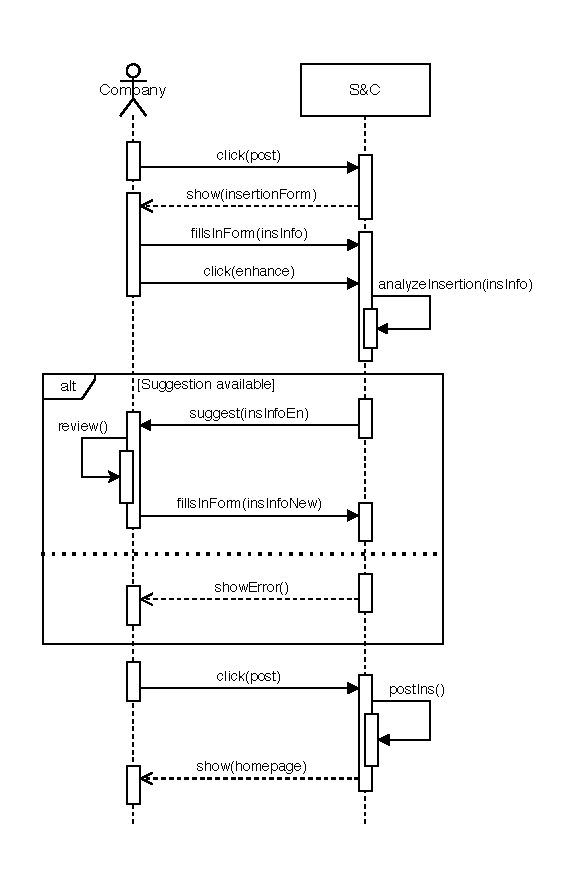
\includegraphics[width=\linewidth]{Images/SequenceDiagram/InsertInternSD2.pdf}
        \caption{Insert an enhanced Internship Insertion sequence diagram.}
        \label{fig:insert_intern_seqdiag}%
    \end{center}
\end{figure}


\subsubsection*{UC\cuc . Enhance CV}
\begin{center}
    \begin{longtable}{|l|p{0.75\linewidth}|}
        \hline
        \textbf{Name}               & Enhance CV\\
        \hline
        \textbf{Actor}              & S\\
        \hline
        \textbf{Entry conditions}   & The S is logged in, has already uploaded a CV and wants to improve it.\\
        \hline
        \textbf{Event Flow}         & 1 - The S opens his personal profile page. \\
        & 2 - The S clicks on the “Enhance” button near the CV section. \\
        & 3 - The system analyzes the CV and gives suggestions on how to improve it. \\
        & 4 - The S reviews suggestions given by the system. \\
        & 5 - The S makes some suggested changes on the file of the CV. \\
        & 6 - The S reuploads a new version of CV. \\
        \hline
        \textbf{Exit condition}   & The system shows the S profile page. \\       
        \hline
        \textbf{Exceptions}       & \begin{itemize}
            \item The CV is very well-done and there are no suggestions available, so the system shows an error message.
        \end{itemize}\\
        \hline
        \caption{Enhance CV use case.}
        \label{tab: enhance_cv_use_case}
    \end{longtable}
\end{center}
 

\begin{figure}[H]
    \begin{center}
        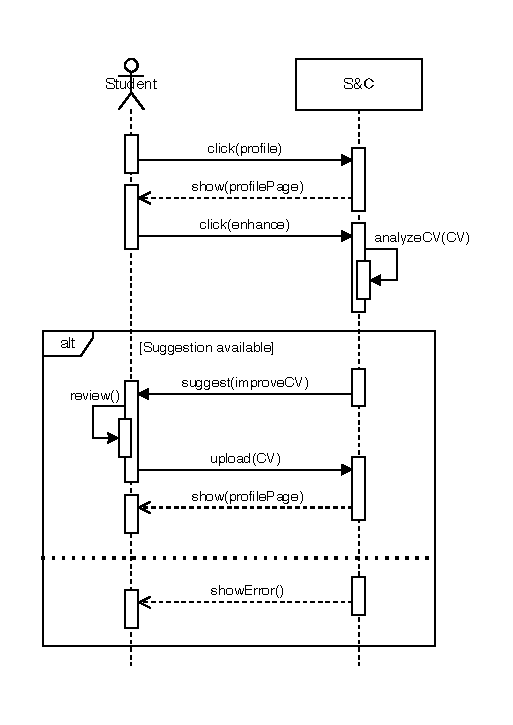
\includegraphics[width=\linewidth]{Images/SequenceDiagram/EnhanceCVSD2.pdf}
        \caption{Enhance CV sequence diagram.}
        \label{fig:enhance_cv_seqdiag}%
    \end{center}
\end{figure}


\subsubsection*{UC\cuc . Submit a feedback}
\begin{center}
    \begin{longtable}{|l|p{0.75\linewidth}|}
        \hline
        \textbf{Name}               & Submit a feedback\\
        \hline
        \textbf{Actor}              & S, C\\
        \hline
        \textbf{Entry conditions}   & The S (C) wants to look for a recommended internship (student) and is on the homepage.\\
        \hline
        \textbf{Event Flow}         & 1 - The S (C) scrolls through the recommended insertions (students). \\
        & 2 - The S (C) clicks on a company’s insertion (student’s profile). \\
        & 3 - The system shows the review of the insertion (student). \\
        & 4 - The S (C) closes the window. \\
        & 5 - The system shows a pop-up asking the S (C) to submit a feedback, including rating and some comments on the received recommendations. \\
        & 6 - The S (C) submits his feedback. \\
        \hline
        \textbf{Exit condition}   & The system saves the feedback to feed the recommendation system and shows the homepage. \\       
        \hline
        \textbf{Exceptions}       & \begin{itemize}
            \item The system does not find any recommended C (S) available for the S (C).
        \end{itemize}\\
        \hline
        \caption{Submit a feedback use case.}
        \label{tab: submit_feedback_use_case}
    \end{longtable}
\end{center}


\begin{figure}[H]
    \begin{center}
        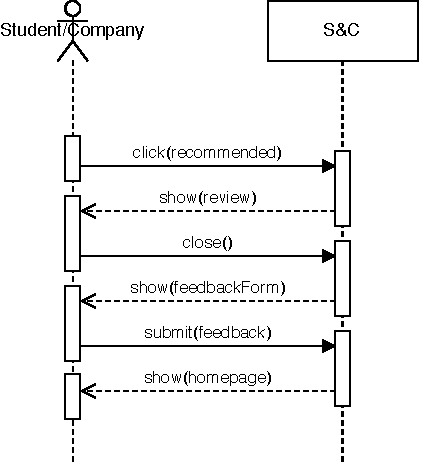
\includegraphics[width=\linewidth]{Images/SequenceDiagram/SubmitFeedbackSD.pdf}
        \caption{Submit a feedback sequence diagram.}
        \label{fig:submit_a_feedback_seqdiag}%
    \end{center}
\end{figure}


\subsubsection*{UC\cuc . Search for a company}
\begin{center}
    \begin{longtable}{|l|p{0.75\linewidth}|}
        \hline
        \textbf{Name}               & Search for a company\\
        \hline
        \textbf{Actor}              & S\\
        \hline
        \textbf{Entry conditions}   & The S is on the homepage and wants to search for a specific C.\\
        \hline
        \textbf{Event Flow}         & 1 - The S clicks on the search bar. \\
        & 2 - The S writes the C’s name and clicks ‘Enter’ on the keyboard or the button ‘Search’. \\
        & 3 - The system shows a list of the matching results. \\
        & 4 - The S clicks on the C profile. \\
        \hline
        \textbf{Exit condition}   & The system shows the C profile. \\       
        \hline
        \textbf{Exceptions}       & \begin{itemize}
            \item The system doesn't find any matching result.
        \end{itemize}\\
        \hline
        \caption{Search for a company use case.}
        \label{tab: search_for_a_company_use_case}
    \end{longtable}
\end{center}


\begin{figure}[H]
    \begin{center}
        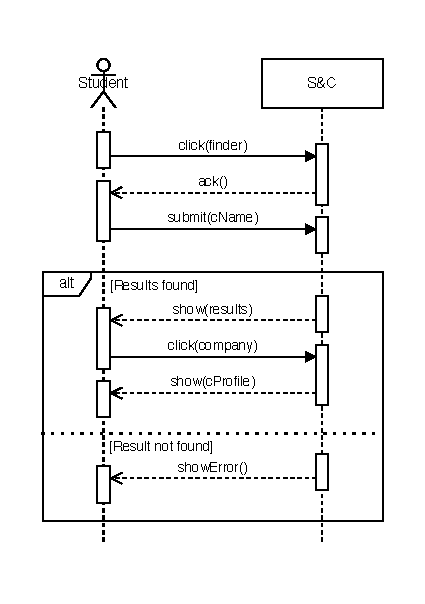
\includegraphics[width=\linewidth]{Images/SequenceDiagram/SearchCompanySD2.pdf}
        \caption{Search for a company sequence diagram.}
        \label{fig:search_for_a_company_seqdiag}%
    \end{center}
\end{figure}


\subsubsection*{UC\cuc . Apply for an internship}
\begin{center}
    \begin{longtable}{|l|p{0.75\linewidth}|}
        \hline
        \textbf{Name}               & Apply for an internship\\
        \hline
        \textbf{Actor}              & S\\
        \hline
        \textbf{Entry conditions}   & The S is logged in and wants to apply for an internship.\\
        \hline
        \textbf{Event Flow}         & 1 - The S finds an interesting insertion. \\
        & 2 - The S clicks on the relative insertion. \\
        & 3 - The system shows the review of the insertion post. \\
        & 4 - The S applies for it, by clicking “Apply”. \\
        \hline
        \textbf{Exit condition}   & The system inserts S into the insertion’s candidates of the C. \\       
        \hline
        \textbf{Exceptions}       & \begin{itemize}
            \item No specific exceptions for this use case.
        \end{itemize}\\
        \hline
        \caption{Apply for an internship use case.}
        \label{tab: apply_for_an_internship_use_case}
    \end{longtable}
\end{center}


\begin{figure}[H]
    \begin{center}
        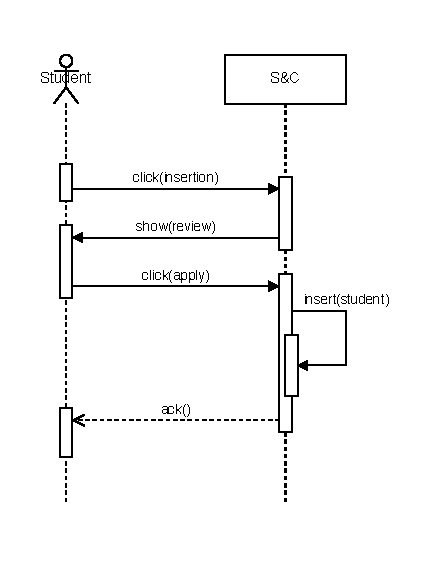
\includegraphics[width=\linewidth]{Images/SequenceDiagram/ApplySD.pdf}
        \caption{Apply for an internship sequence diagram.}
        \label{fig:apply_for_an_internship_seqdiag}%
    \end{center}
\end{figure}


\subsubsection*{UC\cuc . Accept a candidate}
\begin{center}
    \begin{longtable}{|l|p{0.75\linewidth}|}
        \hline
        \textbf{Name}               & Accept a candidate\\
        \hline
        \textbf{Actor}              & C, S, eMail provider\\
        \hline
        \textbf{Entry conditions}   & The C is logged in and wants to find a new candidate from the ones that applied for the internship.\\
        \hline
        \textbf{Event Flow}         & 1 - The C goes on his profile page. \\
        & 2 - The C clicks on "Insertion". \\
        & 3 - The C clicks on the selected insertion post. \\
        & 4 - The system shows the review of the insertion. \\
        & 5 - The C opens the candidates’ section. \\
        & 6 - The C scrolls through all the possible candidates. \\
        & 7 - The C finds a S’s profile. \\
        & 8 - The C clicks on the S’s profile. \\
        & 9 - The system shows the review of the S profile. \\
        & 10 - The C decides to accept the S’s profile by clicking on the “Accept” button. \\
        & 11 - The system sends an eMail to the S notifying him of the decision of the C through the eMail provider. \\
        \hline
        \textbf{Exit condition}   & The system creates a chat between the S and the C. \\       
        \hline
        \textbf{Exceptions}       & \begin{itemize}
            \item There are no candidates available for the internship.
        \end{itemize}\\
        \hline
        \caption{Accept a candidate use case.}
        \label{tab: accept_a_candidate_use_case}
    \end{longtable}
\end{center}


\begin{figure}[H]
    \begin{center}
        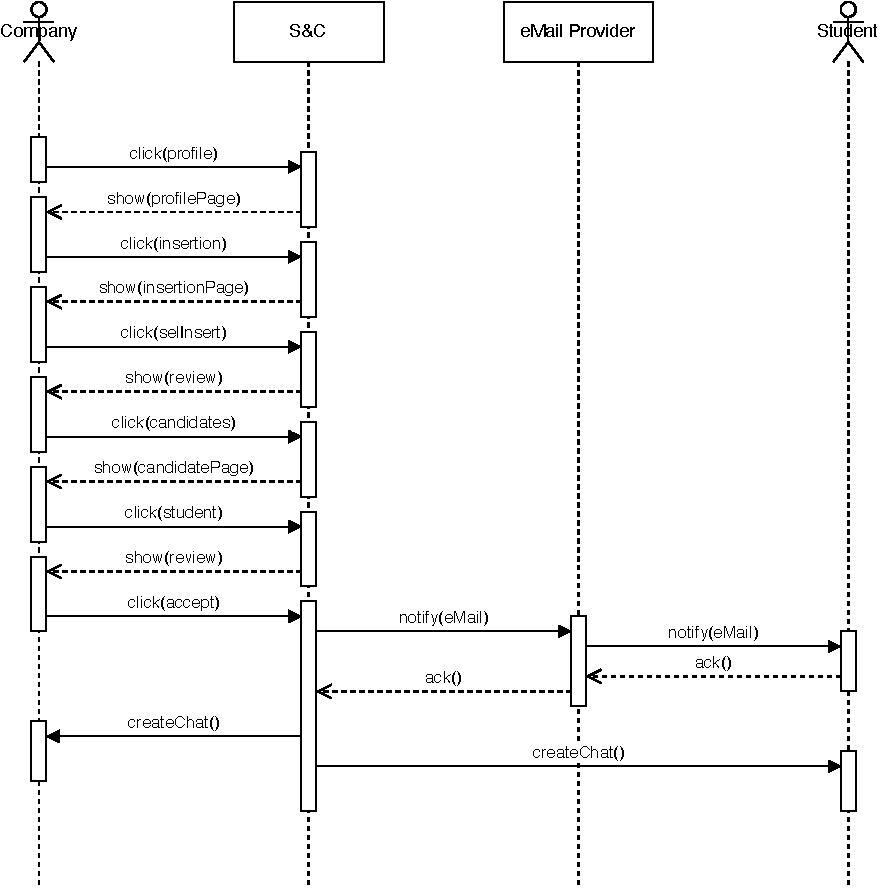
\includegraphics[width=\linewidth]{Images/SequenceDiagram/AcceptCandidateSD.pdf}
        \caption{Accept a candidate sequence diagram.}
        \label{fig:accept_a_candidate_seqdiag}%
    \end{center}
\end{figure}


\subsubsection*{UC\cuc . Submit a Complaint}
\begin{center}
    \begin{longtable}{|l|p{0.75\linewidth}|}
        \hline
        \textbf{Name}               & Submit a Complaint\\
        \hline
        \textbf{Actor}              & S, C, eMail provider\\
        \hline
        \textbf{Entry conditions}   & The S (C) has encountered a problem during the internship period.\\
        \hline
        \textbf{Event Flow}         & 1 - The S (C) goes to the chat page. \\
        & 2 - The S (C) clicks on the chat with the selected C (S). \\
        & 3 - The S (C) clicks on the “+” button. \\
        & 4 - The S (C) clicks on “Submit a Complaint”. \\
        & 5 - The system shows the user a form. \\
        & 6 - The S (C) describes the problem in the form. \\
        & 7 - The S (C) clicks on the “Submit” button. \\
        & 8 - The system checks if the description is not empty. \\
        & 9 - If the problem insertion is not empty the system sends a notification and an eMail through the eMail provider to the S’s U. \\
        \hline
        \textbf{Exit condition}   & The complaint is submitted. \\       
        \hline
        \textbf{Exceptions}       & \begin{itemize}
            \item The user tried to submit an empty form. An error message is shown, inviting the user to describe the problem.
        \end{itemize}\\
        \hline
        \caption{Submit a Complaint use case.}
        \label{tab: submit_a_complaint_use_case}
    \end{longtable}
\end{center}


\begin{figure}[H]
    \begin{center}
        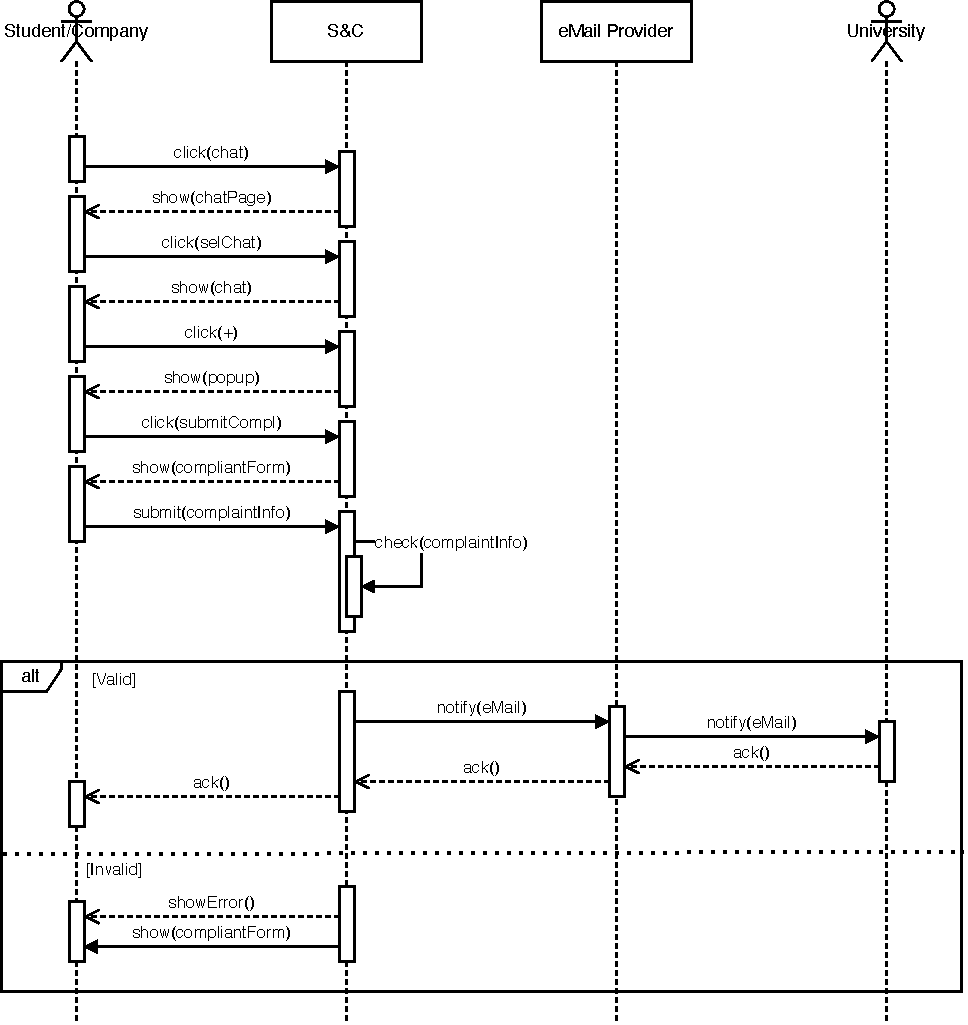
\includegraphics[width=\linewidth]{Images/SequenceDiagram/SubmitComplaintSD.pdf}
        \caption{Submit a Complaint sequence diagram.}
        \label{fig:submit_complaint_seqdiag}%
    \end{center}
\end{figure}


\subsubsection*{UC\cuc . Submit Information}
\begin{center}
    \begin{longtable}{|l|p{0.75\linewidth}|}
        \hline
        \textbf{Name}               & Submit Information\\
        \hline
        \textbf{Actor}              & S, C, eMail provider\\
        \hline
        \textbf{Entry conditions}   & The S (C) has some information to report regarding the ongoing internship.\\
        \hline
        \textbf{Event Flow}         & 1 - The S (C) goes to the chat page. \\
        & 2 - The S (C) clicks on the chat with the selected C (S). \\
        & 3 - The S (C) clicks on the “+” button. \\
        & 4 - The S (C) clicks on “Submit an Information”. \\
        & 5 - The system shows the user a form. \\
        & 6 - The S (C) fills in the form. \\
        & 7 - The S (C) clicks on the “Submit” button. \\
        & 8 - The system checks if the description is not empty. \\
        & 9 - If the information insertion is not empty, the system sends a notification and an eMail through the eMail provider to the S’s U. \\
        \hline
        \textbf{Exit condition}   & The information is submitted. \\       
        \hline
        \textbf{Exceptions}       & \begin{itemize}
            \item The user tried to submit an empty form. An error message is shown, inviting the user to add the information in the form.
        \end{itemize}\\
        \hline
        \caption{Submit Information use case.}
        \label{tab: submit_information_use_case}
    \end{longtable}
\end{center}


\begin{figure}[H]
    \begin{center}
        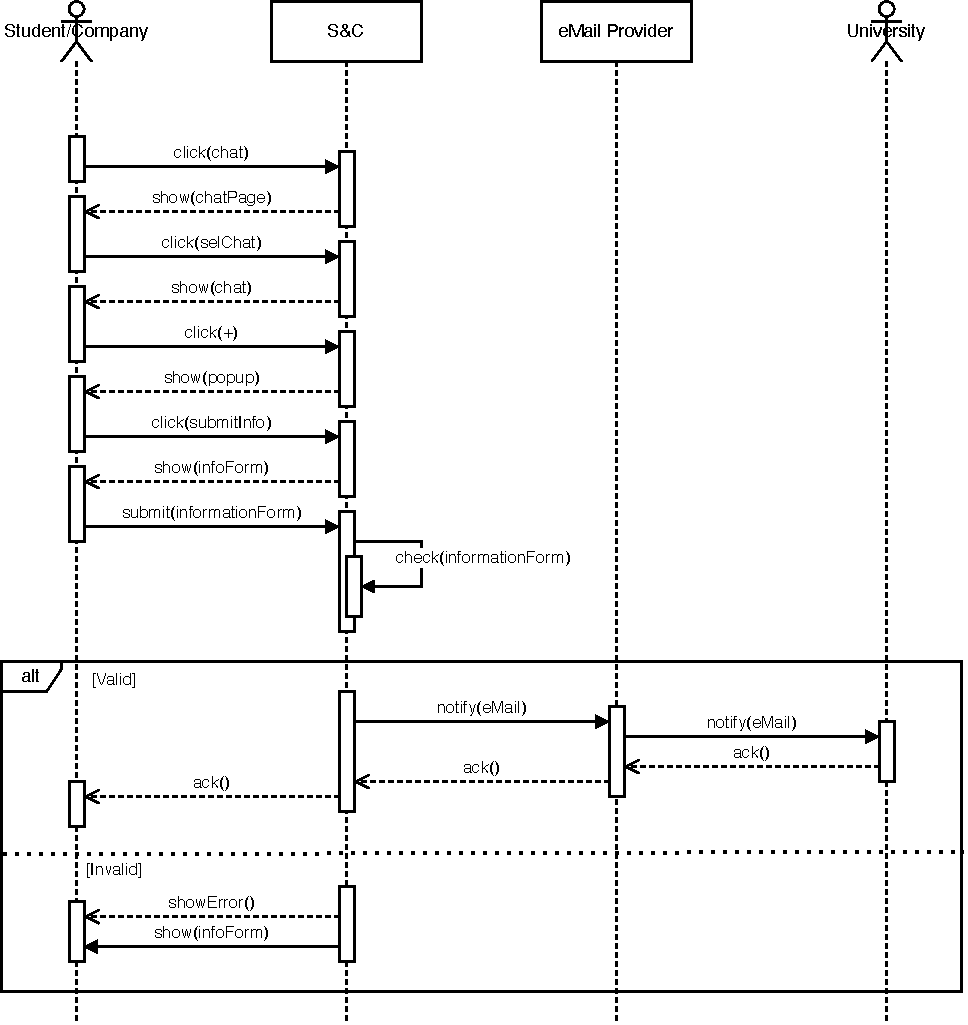
\includegraphics[width=\linewidth]{Images/SequenceDiagram/SubmitInformationSD.pdf}
        \caption{Submit Information sequence diagram.}
        \label{fig:submit_info_seqdiag}%
    \end{center}
\end{figure}


\subsubsection*{UC\cuc . Look for a student through recommended ones}
\begin{center}
    \begin{longtable}{|l|p{0.75\linewidth}|}
        \hline
        \textbf{Name}               & Look for a student through recommended ones\\
        \hline
        \textbf{Actor}              & C\\
        \hline
        \textbf{Entry conditions}   & The C wants to look for a S and has an open position for an internship.\\
        \hline
        \textbf{Event Flow}         & 1 - The C clicks on the profile page. \\
        & 2 - The C clicks on "Insertion". \\
        & 3 - The C selects the internship posting for which it wants to find a candidate. \\
        & 4 - The system shows the review of the insertion. \\
        & 5 - The C opens the candidates’ section. \\
        & 6 - The system shows the recommended students. \\
        \hline
        \textbf{Exit condition}   & The C can look through all the recommended students for that internship. \\       
        \hline
        \textbf{Exceptions}       & \begin{itemize}
            \item There are no recommended S for that internship posting.
        \end{itemize}\\
        \hline
        \caption{Look for a student through recommended ones use case.}
        \label{tab: look_for_student_use_case}
    \end{longtable}
\end{center}


\begin{figure}[H]
    \begin{center}
        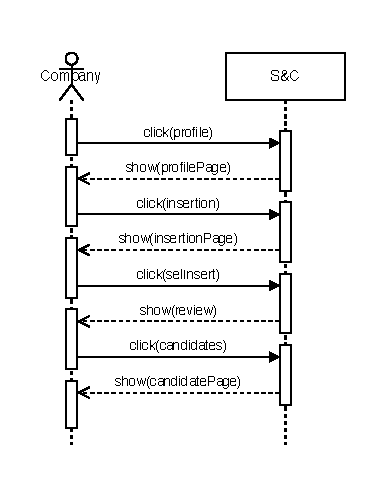
\includegraphics[width=\linewidth]{Images/SequenceDiagram/LookStudentSD2.pdf}
        \caption{Look for a student through recommended ones sequence diagram.}
        \label{fig:look_student_seqdiag}%
    \end{center}
\end{figure}


\subsubsection*{UC\cuc . Contact a recommended student}
\begin{center}
    \begin{longtable}{|l|p{0.75\linewidth}|}
        \hline
        \textbf{Name}               & Contact a recommended student\\
        \hline
        \textbf{Actor}              & C, S, eMail provider\\
        \hline
        \textbf{Entry conditions}   & The C wants to send the proposal for an internship to a recommended student.\\
        \hline
        \textbf{Event Flow}         & 1 - The C clicks on the profile page. \\
        & 2 - The C selects the internship posting for which it wants to find a candidate. \\
        & 3 - The C starts scrolling through the recommended student’s profiles. \\
        & 4 - The C clicks on the profile of a recommended S. \\
        & 5 - The C reviews the S’s CV. \\
        & 6 - The C contacts the S, by clicking “Contact”. \\
        & 7 - The system sends a notification and an eMail through the eMail provider to the S. \\
        \hline
        \textbf{Exit condition}   & The S receives a contact request from the C. \\       
        \hline
        \textbf{Exceptions}       & \begin{itemize}
            \item There are no recommended students for the internship.
        \end{itemize}\\
        \hline
        \caption{Contact a recommended student use case.}
        \label{tab: contact_recommended_student_use_case}
    \end{longtable}
\end{center}


\begin{figure}[H]
    \begin{center}
        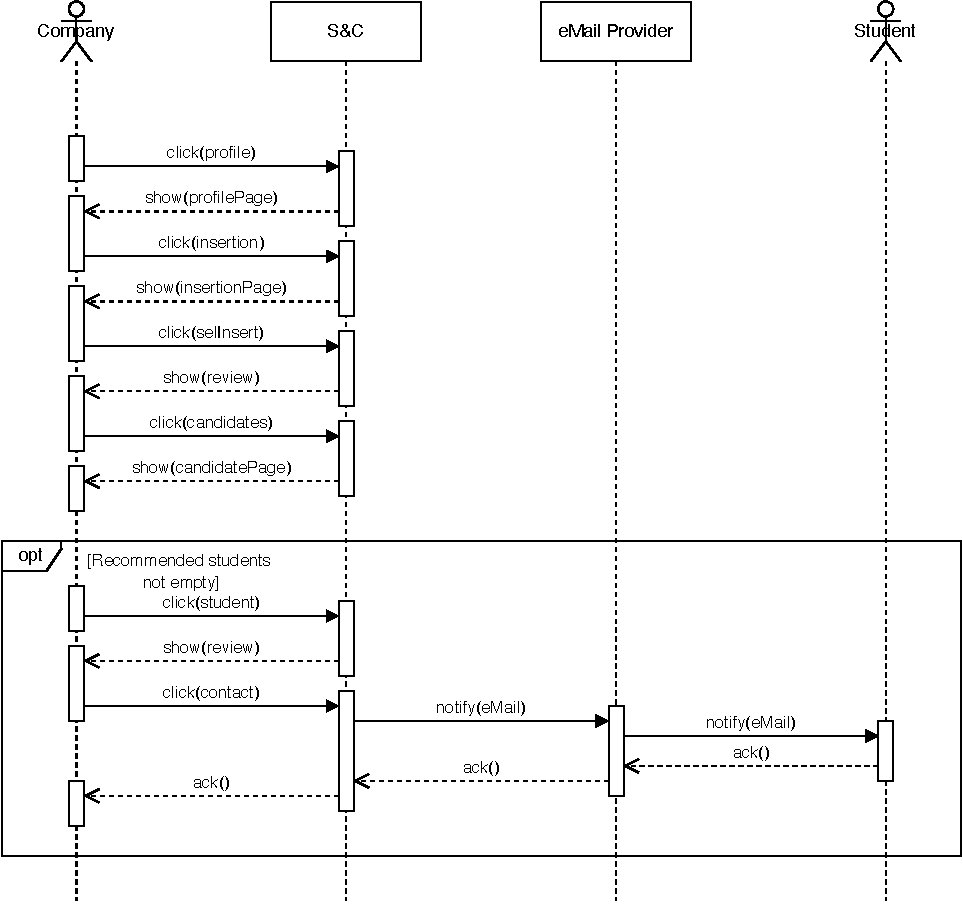
\includegraphics[width=\linewidth]{Images/SequenceDiagram/ContactStudentSD.pdf}
        \caption{Contact a recommended student sequence diagram.}
        \label{fig:contact_student_seqdiag}%
    \end{center}
\end{figure}


\subsubsection*{UC\cuc . Accept a company}
\begin{center}
    \begin{longtable}{|l|p{0.75\linewidth}|}
        \hline
        \textbf{Name}               & Accept a company\\
        \hline
        \textbf{Actor}              & S, C, eMail provider\\
        \hline
        \textbf{Entry conditions}   & The C has contacted the S proposing him an internship position and the S wants to accept it.\\
        \hline
        \textbf{Event Flow}         & 1 - The S goes on his notification page. \\
        & 2 - The S scrolls through the list of C that contacted him. \\
        & 3 - The S clicks on the C’s profile and reviews the internship description. \\
        & 4 - The S decides to accept the internship by clicking on the “Accept” button. \\
        & 5 - An email is sent to the C through the eMail provider, notifying them that the student accepted their request. \\
        \hline
        \textbf{Exit condition}   & The system creates a chat between the S and the C. \\       
        \hline
        \caption{Accept a company use case.}
        \label{tab: accept_company_use_case}
    \end{longtable}
\end{center}


\begin{figure}[H]
    \begin{center}
        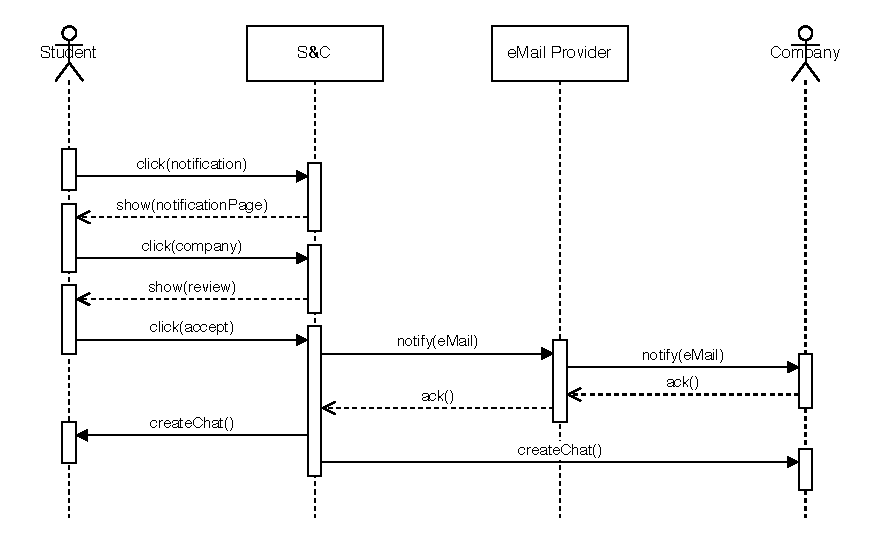
\includegraphics[width=\linewidth]{Images/SequenceDiagram/AcceptCompanySD.pdf}
        \caption{Accept a company sequence diagram.}
        \label{fig:accept_company_seqdiag}%
    \end{center}
\end{figure}


\subsubsection*{UC\cuc . Schedule an Interview}
\begin{center}
    \begin{longtable}{|l|p{0.75\linewidth}|}
        \hline
        \textbf{Name}               & Schedule an Interview\\
        \hline
        \textbf{Actor}              & S, C\\
        \hline
        \textbf{Entry conditions}   & The S and the C have accepted each other’s request and a chat is established between them.\\
        \hline
        \textbf{Event Flow}         & 1 - The C clicks on the “+” button. \\
        & 2 - The C selects “schedule interview”. \\
        & 3 - The C compiles a form selecting a date and time for the interview. \\
        & 4 - The C submits the form and sends it to the S. \\
        & 5 - The S can either accept or decline the proposal by selecting the appropriate option. \\
        & 6 - If the S accepts, the event is added to the S\&C calendar for both the S and the C. \\
        \hline
        \textbf{Exit condition}   & An interview event is scheduled and added to both the S’s and the C’s S\&C calendars. \\       
        \hline
        \textbf{Exceptions}       & The S declines the interview proposal from the C, and the system cancel the proposal. \\
        \hline
        \caption{Schedule an Interview use case.}
        \label{tab: schedule_interview_use_case}
    \end{longtable}
\end{center}


\begin{figure}[H]
    \begin{center}
        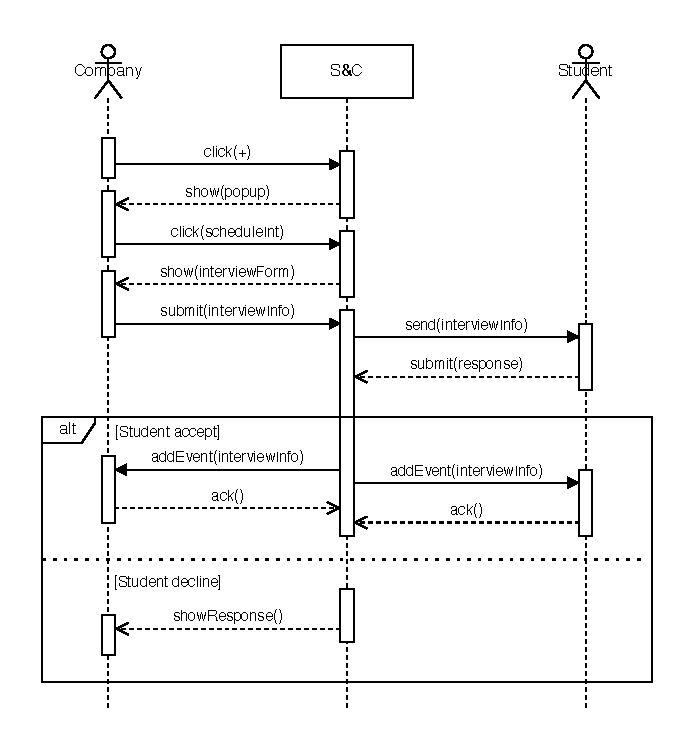
\includegraphics[width=\linewidth]{Images/SequenceDiagram/ScheduleInterviewSD.pdf}
        \caption{Schedule an Interview sequence diagram.}
        \label{fig:schedule_interview_seqdiag}%
    \end{center}
\end{figure}


\subsubsection*{UC\cuc . Start an Internship}
\begin{center}
    \begin{longtable}{|l|p{0.75\linewidth}|}
        \hline
        \textbf{Name}               & Start an Internship\\
        \hline
        \textbf{Actor}              & S, C\\
        \hline
        \textbf{Entry conditions}   & The S and the C have already completed an interview, and the C is impressed with the S.\\
        \hline
        \textbf{Event Flow}         & 1 - The C clicks on the “+” button. \\
        & 2 - The C selects “propose internship”. \\
        & 3 - The C compiles a form selecting the dates of starting and ending of the internship. \\
        & 4 - The C submits the form and sends it to the S. \\
        & 5 - The S accepts the proposal by selecting the appropriate option. \\
        \hline
        \textbf{Exit condition}   & The system adds the event to both the S’s and the C’s S\&C calendars. \\       
        \hline
        \textbf{Exceptions}       & The S declines the offer and the chat between S and C is closed. \\
        \hline
        \caption{Start an Internship use case.}
        \label{tab: start_internship_use_case}
    \end{longtable}
\end{center}


\begin{figure}[H]
    \begin{center}
        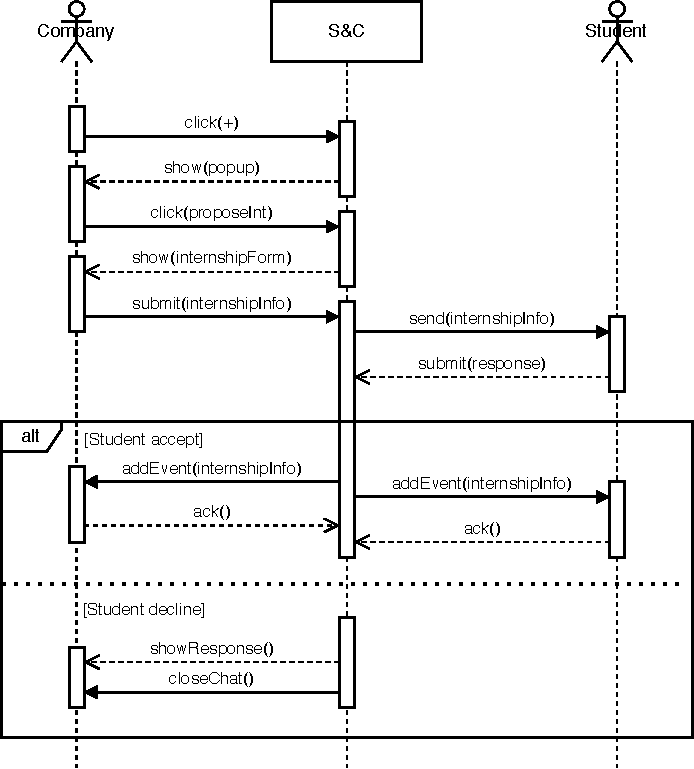
\includegraphics[width=\linewidth]{Images/SequenceDiagram/StartInternSD.pdf}
        \caption{Start an Internship sequence diagram.}
        \label{fig:start_internship_seqdiag}%
    \end{center}
\end{figure}


\subsubsection*{UC\cuc . Monitor internship}
\begin{center}
    \begin{longtable}{|l|p{0.75\linewidth}|}
        \hline
        \textbf{Name}               & Monitor internship\\
        \hline
        \textbf{Actor}              & U\\
        \hline
        \textbf{Entry conditions}   & The U monitors the internship between the C and the S.\\
        \hline
        \textbf{Event Flow}         & 1 - The U goes on the main page. \\
        & 2 - The U clicks on the chat regarding the S and the C. \\
        & 3 - The system shows the chat and the related complaints or information. \\
        \hline
        \textbf{Exit condition}   & The U can monitor the information and issues reported by the other two parties during the internship. \\       
        \hline
        \caption{Monitor Internship use case.}
        \label{tab: monitor_internship_use_case}
    \end{longtable}
\end{center}


\begin{figure}[H]
    \begin{center}
        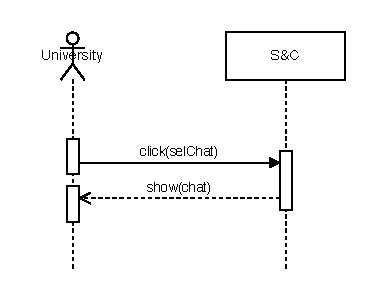
\includegraphics[width=\linewidth]{Images/SequenceDiagram/MonitorInternSD.pdf}
        \caption{Monitor Internship sequence diagram.}
        \label{fig:monitor_intern_seqdiag}%
    \end{center}
\end{figure}


\subsubsection*{UC\cuc . Interrupt internship}
\begin{center}
    \begin{longtable}{|l|p{0.75\linewidth}|}
        \hline
        \textbf{Name}               & Interrupt internship\\
        \hline
        \textbf{Actor}              & U, S, C, eMail provider\\
        \hline
        \textbf{Entry conditions}   & The U monitors the internship and reads a complaint.\\
        \hline
        \textbf{Event Flow}         & 1 - The U goes on the main page. \\
        & 2 - The U clicks on the related chat. \\
        & 3 - The U reviews the complaint. \\
        & 4 - If the U deems it necessary, clicks on “Interrupt Internship”. \\
        & 5 - The system sends an eMail through the eMail provider and notifies the S and C about the interruption of the internship. \\
        \hline
        \textbf{Exit condition}   & The internship is interrupted and the chat closed. \\       
        \hline
        \caption{Interrupt internship use case.}
        \label{tab: interrupt_internship_use_case}
    \end{longtable}
\end{center}


\begin{figure}[H]
    \begin{center}
        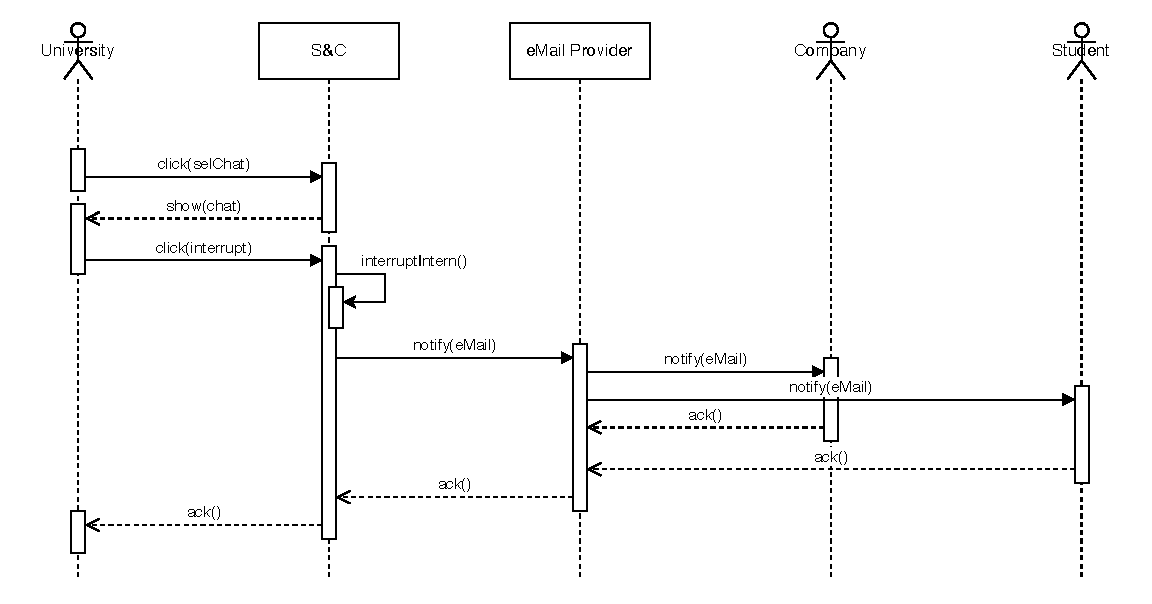
\includegraphics[width=\linewidth]{Images/SequenceDiagram/InterruptInternSD.pdf}
        \caption{Interrupt Internship sequence diagram.}
        \label{fig:interrupt_intern_seqdiag}%
    \end{center}
\end{figure}



\subsection{Mapping on goals}
\label{subsec:mapping_on_goals}%

The mapping links the platform's goals to specific
requirements and domain assumptions, ensuring each objective is
addressed effectively.

\begin{itemize}
\item
  \textbf{{[}G1{]}: University students would like to seek internships
  that better align with their interests and field of study.}

  \begin{itemize}
  \item
    {[}R1{]}: The system should allow an unregistered guest to sign up.
  \item
    {[}R2{]}: The system should allow registered students to log in.
  \item
    {[}R3{]}: The system should allow students to insert their CVs and
    manage their profile information (e.g. personal data, skills and
    profile photo).
  \item
    {[}R4{]}: The system should provide personalized suggestions to
    students for enhancing their CVs to improve their chances of being
    selected.
  \item
    {[}R5{]}: The system should notify students when internships
    matching their skills, experiences, and interests become available.
  \item
    {[}R6{]}: The system should allow students to browse available
    internship postings.
  \item
    {[}R7{]}: The system allows S to visualize the profile of other C.~
  \item
    {[}R8{]}: The system should allow S to submit applications for
    specific internship postings.
  \item
    {[}D1{]} S must be enrolled in a U.
  \item
    {[}D3{]} S should already have a valid Cv to be uploaded.
  \item
    {[}D4{]} S's Cv should be a PDF document.
  \item
    {[}D5{]} The User can easily access his eMail provider.
  \item
    {[}D6{]} S,C provide accurate and truthful information in their
    profiles, CVs, and internship description.
  \item
    {[}D9{]} The S\&C recommendation engine achieves high accuracy when
    S and C provide detailed, complete, and accurate information in
    their CVs and job descriptions.
  \item
    {[}D10{]} The AI system integrated into the S\&C platform
    effectively enhances students' CVs and
    companies' internship postings, providing accurate
    and useful suggestions to improve the matching process.
  \item
    {[}D11{]} The eMail provider functions reliably, ensuring that all
    emails, including verification and notification messages, are
    successfully delivered to the intended recipients.
  \end{itemize}
\end{itemize}

\begin{itemize}
\item
  \textbf{{[}G2{]}: Companies would like to offer internships to
  students who best match the related figure.}

  \begin{itemize}
  \item
    {[}R1{]}: The system should allow an unregistered guest to sign up.
  \item
    {[}R16{]}: The system should allow registered companies to log in.
  \item
    {[}R17{]}: The system should allow C to manage their organization
    profile.
  \item
    {[}R18{]}: The system should allow C to post new internship
    opportunities, specifying details such as required skills, tasks,
    and benefits.
  \item
    {[}R19{]}: The system should provide suggestions to C to improve
    their internship postings, making them more appealing to S.
  \item
    {[}R20{]}: The system allows C to visualize the profile of other
    Users.
  \item
    {[}R21{]}: The system should inform C about the availability of S
    CVs corresponding to their needs.
  \item
    {[}R23{]}: The system allows C to establish a contact with S when
    mutual interest is identified.
  \item
    {[}D5{]} The User can easily access his eMail provider.
  \item
    {[}D6{]} S,C provide accurate and truthful information in their
    profiles, CVs, and internship description.
  \item
    {[}D8{]} C on the platform are assumed to be legitimate and offer
    genuine internships, operating legally and ethically without
    verification by S\&C.
  \item
    {[}D9{]} The S\&C recommendation engine achieves high accuracy when
    S and C provide detailed, complete, and accurate information in
    their CVs and job descriptions.
  \item
    {[}D10{]} The AI system integrated into the S\&C platform
    effectively enhances students' CVs and
    companies' internship postings, providing accurate
    and useful suggestions to improve the matching process.
  \item
    {[}D11{]} The eMail provider functions reliably, ensuring that all
    emails, including verification and notification messages, are
    successfully delivered to the intended recipients.
  \end{itemize}
\end{itemize}

\begin{itemize}
\item
  \textbf{{[}G3{]}: Enhance communication and coordination between
  students and companies in the selection process.}

  \begin{itemize}
  \item
    {[}R2{]}: The system should allow registered students to log in.
  \item
    {[}R10{]}: The system allows S to establish a contact with C when
    mutual interest is identified.
  \item
    {[}R11{]}: The system should assist S in scheduling interviews.
  \item
    {[}R12{]}: The system should allow S to track the status of their
    applications and final selections.
  \item
    {[}R14{]}: The system should allow S to review the S\&C Calendar.
  \item
    {[}R15{]}: The system should insert the S's events on the S\&C
    Calendar.
  \item
    {[}R16{]}: The system should allow registered companies to log in.
  \item
    {[}R23{]}: The system allows C to establish a contact with S when
    mutual interest is identified.
  \item
    {[}R24{]}: The system should enable C to track the progress of their
    internship selection processes, including applications and
    decisions.~
  \item
    {[}R26{]}: The system should allow C to review the S\&C Calendar.
  \item
    {[}R27{]}: The system should insert the C's events on the S\&C
    Calendar.
  \item
    {[}D12{]} Students and companies are committed to the internship
    process and will engage with features such as scheduling interviews
    and responding to feedback.
  \item
    {[}D13{]} Companies must clearly communicate interview requirements
    (e.g., time, format, platform) to students during scheduling.
  \item
    {[}D14{]} Interviews must be conducted either in person or via
    secure external tools, with students and companies responsible for
    ensuring their availability and functionality.
  \end{itemize}
\end{itemize}

\begin{itemize}
\item
  \textbf{{[}G4{]}: Evolve the recommendation system through feedback
  and suggestions (provided by students and companies) to improve future
  matches.}

  \begin{itemize}
  \item
    {[}R2{]}: The system should allow registered students to log in.
  \item
    {[}R5{]}: The system should notify students when internships
    matching their skills, experiences, and interests become available.
  \item
    {[}R7{]}: The system allows S to visualize the profile of other C.~
  \item
    {[}R9{]}: The system should allow S to provide feedback, suggestions
    and rating to improve the recommendation process.
  \item
    {[}R16{]}: The system should allow registered companies to log in.
  \item
    {[}R20{]}: The system allows C to visualize the profile of other
    Users.
  \item
    {[}R21{]}: The system should inform C about the availability of S
    CVs corresponding to their needs.
  \item
    {[}R22{]}: The system should allow C to provide feedback and
    suggestions to improve the recommendation process.
  \item
    {[}D6{]} S,C provide accurate and truthful information in their
    profiles, CVs, and internship description.
  \item
    {[}D9{]} The S\&C recommendation engine achieves high accuracy when
    S and C provide detailed, complete, and accurate information in
    their CVs and job descriptions.
  \item
    {[}D10{]} The AI system integrated into the S\&C platform
    effectively enhances students' CVs and
    companies' internship postings, providing accurate
    and useful suggestions to improve the matching process.
  \item
    {[}D12{]} Students and companies are committed to the internship
    process and will engage with features such as scheduling interviews
    and responding to feedback.
  \end{itemize}
\end{itemize}

\begin{itemize}
\item
  \textbf{{[}G5{]}: Universities would like to monitor internships and
  handle any emerging issues promptly, ensuring a smooth and beneficial
  experience for all parties involved.}

  \begin{itemize}
  \item
    {[}R1{]}: The system should allow an unregistered guest to sign up.
  \item
    {[}R13{]}: The system should provide S with a mechanism to report
    issues or complaints related to ongoing internships.
  \item
    {[}R25{]}: The system should allow C to submit complaints or
    information related to internships.
  \item
    {[}R28{]}: The system should allow U to log in.
  \item
    {[}R29{]}: The system should allow U to monitor internships of their
    students.
  \item
    {[}R30{]}: The system should allow U to interrupt ongoing
    internships.
  \item
    {[}D2{]} The related U should be already registered when the S signs
    up.
  \item
    {[}D5{]} The User can easily access his eMail provider.
  \item
    {[}D7{]} U are willing and able to use the S\&C platform to monitor
    internship statuses, address complaints, and respond to student or
    company feedback as needed.
  \item
    {[}D11{]} The eMail provider functions reliably, ensuring that all
    emails, including verification and notification messages, are
    successfully delivered to the intended recipients.
  \end{itemize}
\end{itemize}

\begin{longtable}{|l|c|c|c|c|c|l|}
\hline
\textbf{Requirements and Domain Assumption} & \textbf{G1} & \textbf{G2} & \textbf{G3} & \textbf{G4} & \textbf{G5} & \textbf{UC} \\
\hline
\endfirsthead
\hline
\textbf{Requirements and Domain Assumption} & \textbf{G1} & \textbf{G2} & \textbf{G3} & \textbf{G4} & \textbf{G5} & \textbf{UC} \\
\hline
\endhead
R1  & X & X &   &   & X & UC1  \\
\hline
R2  & X &   & X & X &   & UC2  \\
\hline
R3  & X &   &   &   &   &       \\
\hline
R4  & X &   &   &   &   &       \\
\hline
R5  & X &   &   & X &   &       \\
\hline
R6  & X &   &   &   &   &       \\
\hline
R7  & X &   &   & X &   &       \\
\hline
R8  & X &   &   &   &   &       \\
\hline
R9  &   &   &   & X &   &       \\
\hline
R10 &   &   & X &   &   &       \\
\hline
R11 &   &   & X &   &   &       \\
\hline
R12 &   &   & X &   &   &       \\
\hline
R13 &   &   &   &   & X &       \\
\hline
R14 &   &   & X &   &   &       \\
\hline
R15 &   &   & X &   &   &       \\
\hline
R16 &   & X & X & X &   & UC2   \\
\hline
R17 &   & X &   &   &   &       \\
\hline
R18 &   & X &   &   &   &       \\
\hline
R19 &   & X &   &   &   &       \\
\hline
R20 &   & X &   & X &   &       \\
\hline
R21 &   & X &   & X &   &       \\
\hline
R22 &   &   &   & X &   &       \\
\hline
R23 &   & X & X &   &   &       \\
\hline
R24 &   &   & X &   &   &       \\
\hline
R25 &   &   &   &   & X &       \\
\hline
R26 &   &   & X &   &   &       \\
\hline
R27 &   &   & X &   &   &       \\
\hline
R28 &   &   &   &   & X &       \\
\hline
R29 &   &   &   &   & X &       \\
\hline
R30 &   &   &   &   & X &       \\
\hline
D1  & X &   &   &   &   &       \\
\hline
D2  &   &   &   &   & X &       \\
\hline
D3  & X &   &   &   &   &       \\
\hline
D4  & X &   &   &   &   &       \\
\hline
D5  & X & X &   &   & X &       \\
\hline
D6  & X & X &   & X &   &       \\
\hline
D7  &   &   &   &   & X &       \\
\hline
D8  &   & X &   &   &   &       \\
\hline
D9  & X & X &   & X &   &       \\
\hline
D10 & X & X &   & X &   &       \\
\hline
D11 & X & X &   &   & X &       \\
\hline
D12 &   &   & X & X &   &       \\
\hline
D13 &   &   & X &   &   &       \\
\hline
D14 &   &   & X &   &   &       \\
\hline
\caption{Traceability Matrix of Requirements and Domain Assumptions to Goals and Use Cases}
\label{tab:mapping_requirements_domain_assumptions}
\end{longtable}


\section{Performance requirements}
\label{sec:performance_requirements}%


\paragraph{Number of Concurrent Users:}
  The S\&C platform must be designed to handle a significant number of
  concurrent users, ensuring smooth performance even during peak
  activity periods, such as internship application deadlines. The
  platform should support a substantial portion of its active user base
  accessing the system simultaneously.
\paragraph{Data Storage:}
  The platform must store and manage all relevant information about
  students, including CVs, profiles, and application statuses, as well
  as companies' internship postings, feedback, and selection processes.
  Historical data, such as completed internships and feedback, should
  remain accessible to support recommendations and user references.
\paragraph{Response Time:}
  Operations directly executed by the S\&C platform, such as
  registration, login, posting internships, applying for internships,
  and scheduling interviews, must have a response time of under 500
  milliseconds. For operations involving external systems, such as email
  notifications or third-party scheduling tools, the platform will
  strive to minimize delays but cannot guarantee their performance.

\section{Design constraints}
\label{sec:design_constraints}%


\subsection{Standard compliance}
\label{subsec:standard compliance}%%


The S\&C platform must comply with relevant data protection and privacy
regulations, including the EU's General Data Protection Regulation
(GDPR). This regulation ensures that the personal data of users,
including students, companies, and universities, is collected, stored,
and processed securely and transparently. The platform must implement
appropriate measures to protect user privacy and ensure data security.


\subsection{Hardware limitations}
\label{subsec:hardware_limitations}%


The primary hardware requirement for accessing the S\&C platform is a
reliable internet connection and a device with a modern web browser.


\section{Software system attributes}
\label{sec:software_system_attributes}%


\subsection{Reliability}
\label{subsec:reliability}%


The S\&C platform must be fault-tolerant to ensure continuous service
and minimize the impact of potential errors. This will prevent system
failures from propagating, allowing users to continue their tasks
without significant interruptions.


\subsection{Availability}
\label{subsec:availability}%


The S\&C platform must maintain a high level of availability. This
ensures that the platform is accessible to users at all times,
minimizing disruption to their internship search and application
processes.~


\subsection{Security}
\label{subsec:security}%


The platform must implement robust security measures to protect user
data and ensure secure access. This includes both authentication and
authorization:

\begin{itemize}
\item
  Authentication will verify the identity of users attempting to log in,
  ensuring only legitimate users can access the platform.
\item
  Authorization will manage the permissions of authenticated users,
  restricting access to specific features based on user roles (e.g.,
  students, companies, or universities).
\end{itemize}

To protect sensitive information, the system will adopt best practices
for data security, including:

\begin{itemize}
\item
  Encryption of passwords and personal data stored in the database.
\item
  Protection against query injections and other common security
  vulnerabilities to prevent unauthorized data access.
\end{itemize}

These measures will ensure that the system maintains a secure
environment for users and their data.


\subsection{Maintainability}
\label{subsec:maintainability}%


The S\&C platform must be designed using scalable and modular components
to allow easy updates and additions of new features with minimal effort.
The architecture should support future expansions, such as new
functionalities or integrations with third-party services, without major
changes to the core system. Regular maintenance should be scheduled
during off-peak hours, preferably at night, to ensure minimal disruption
to users during peak traffic periods.


\subsection{Portability}
\label{subsec:portability}%


The system must be accessible to users from any device or platform that
supports a modern web browser. This ensures that students, companies,
and universities can access the platform from a variety of devices. On
the server side, there are no specific portability requirements, as the
platform will rely on standard web technologies and services to ensure
compatibility across different environments.